\documentclass[letter,12pt]{article}
\usepackage[left=2.54cm, right=2.54cm, top=2.54cm, bottom=2.54cm]{geometry} % Márgenes APA
\usepackage{setspace} % Interlineado
\setlength{\parindent}{1.27cm} % Sangría estándar APA
\setlength{\parskip}{0pt}     % Sin espacio entre párrafos
\usepackage{graphicx} % Para insertar imágenes
\usepackage{float} % Para posicionar imágenes y tablas
\usepackage{caption} % Para modificar captions de tablas e imágenes
\usepackage{csquotes} % Para mejor manejo de citas
\usepackage{amsmath} % Para ecuaciones matemáticas
\usepackage{svg}
\usepackage{indentfirst}
\usepackage[utf8]{inputenc} % Soporte para UTF-8
\usepackage[T1]{fontenc}    % Codificación de fuente
\usepackage{textcomp}       % Símbolos adicionales (≈)
\usepackage{tabularx} % <-- Añadir al preámbulo si no está
\usepackage{longtable} % Añadir al preámbulo si no está
% \usepackage{ltablex} % Añadir al preámbulo si no está
% \keepXColumns % Para que X funcione igual que en tabularx

%==========REFERENCIAS=============
\usepackage[backend=bibtex,style=ieee,language=spanish]{biblatex}
\addbibresource{referencias.bib}

\usepackage[
    pdftitle={Tarea \# 1 - FFT y Sistemas de Modulación}, % Título del PDF
    pdfauthor={Barquero, J., Feng, J., Montero, A.},   % Autor del PDF
    pdfsubject={CE1110 - Análisis de Señales Mixtas}, % Tema del PDF
    pdfkeywords={}, % Palabras clave del PDF
    pdfproducer={LaTeX with hyperref package},
    pdfcreator={pdfLatex}
]{hyperref}

\hypersetup{
    colorlinks=true,        % Colorea los enlaces en lugar de usar cajas alrededor de ellos
    linkcolor = black,
    urlcolor  = blue,
    citecolor = black,
    anchorcolor = blue         % Color de los enlaces externos
}

\begin{document}
% ====== Portada ======
\begin{titlepage}
    \centering
    {\LARGE \textbf{Tarea \# 1} \par}
    {\LARGE FFT y Sistemas de Modulación \par}
    \vspace{1.5cm}
    {\large José Bernardo Barquero Bonilla \\ 2023150476 \par}
    {\large Jimmy Feng Feng \\ 2023060347 \par}
    {\large Alexander Montero Vargas \\ 2023166058 \par}
    \vspace{1.5cm}
    {\Large Instituto Tecnológico de Costa Rica \par}
    {\large Escuela de Ingeniería en Computadores \par}
    {\large Curso: CE1110 - Análisis de Señales Mixtas \par}
    \vspace{1.5cm}
    {\large Profesor: Luis Alberto Chavarría Zamora \par}
    \vfill
    {\large 15 de Octubre de 2025 \par}
\end{titlepage}

% ====== Desarrollo ======
\section{DFT/FFT y serie de Fourier}

La Transformada Discreta de Fourier (DFT) es la definición matemática que proyecta una secuencia finita \(x[n]\) de longitud \(N\) sobre exponenciales complejas y entrega \(N\) muestras espectrales \(X[k]\) igualmente espaciadas en frecuencia \cite{OppenheimSchaferDTSP3e,VetterliKovacevicGoyalFSP2014}. La DFT se calcula como
\[
X[k]=\sum_{n=0}^{N-1} x[n]\,e^{-j2\pi kn/N},\quad k=0,\dots,N-1,
\]
y la inversa como
\[
x[n]=\frac{1}{N}\sum_{k=0}^{N-1} X[k]\,e^{+j2\pi kn/N},\quad n=0,\dots,N-1.
\]
Estas expresiones fijan la convención de normalización usada a lo largo del documento \cite{OppenheimSchaferDTSP3e}.

La Transformada Rápida de Fourier (FFT) no es una transformada distinta, sino un algoritmo que evalúa la DFT con complejidad \(O(N\log N)\), en contraste con los \(O(N^2)\) de la evaluación directa \cite{CooleyTukey1965}. En la práctica, “hacer una FFT” significa calcular la DFT de forma eficiente; la distinción es: \emph{qué} se calcula (DFT) versus \emph{cómo} se calcula (FFT) \cite{OppenheimSchaferDTSP3e,NumPyFFT2024}.

Para una señal discreta \(x[n]\), la transformada \(X(e^{j\omega})\) (DTFT) es continua en \(\omega\) y periódica con período \(2\pi\) \cite{OppenheimSchaferDTSP3e,NISTDLMF_Fourier}:
\[
X(e^{j\omega})=\sum_{n=-\infty}^{\infty} x[n]\,e^{-j\omega n},\qquad
X(e^{j(\omega+2\pi)})=X(e^{j\omega}).
\]
La DFT puede interpretarse como un \emph{muestreo} de esta DTFT en \(N\) frecuencias uniformemente espaciadas \( \omega_k=2\pi k/N \), o en Hz \( f_k=\tfrac{k}{N}f_s \), con resolución \(\Delta f=\tfrac{f_s}{N}\) \cite{OppenheimSchaferDTSP3e,VetterliKovacevicGoyalFSP2014,SciPyFFT2024}. Aumentar \(N\) mejora la resolución; el \emph{zero-padding} densifica la grilla de lectura sin aumentar la resolución física \cite{SciPyFFT2024,NumPyFFT2024}.

La relación con la serie de Fourier surge de la periodicidad. La serie de Fourier representa una señal periódica continua \(x(t)\) como suma de armónicos discretos \(k f_0\) con coeficientes \(c_k\) \cite{OsgoodFTAMS2019,NISTDLMF_Fourier}:
\[
x(t)=\sum_{k=-\infty}^{\infty} c_k\,e^{j2\pi k f_0 t},\qquad
c_k=\frac{1}{T_0}\int_{0}^{T_0} x(t)\,e^{-j2\pi k f_0 t}\,dt.
\]
Análogamente, al tomar un bloque de \(N\) muestras y asumir su repetición periódica en tiempo discreto, la DFT entrega los coeficientes de la serie de Fourier de esa señal periódica discreta: tiempo (discreto) periódico \(\Rightarrow\) espectro (discreto) en \(N\) líneas \cite{OppenheimSchaferDTSP3e,VetterliKovacevicGoyalFSP2014}.

Finalmente, respecto al “muestreo del entorno continuo”, muestrear \(x(t)\) cada \(T_s\) genera \(x[n]=x(nT_s)\) y replica el espectro continuo \(X_c(f)\) cada \(f_s=1/T_s\); si \(f_s<2f_{\max}\) ocurre aliasing \cite{OppenheimSchaferDTSP3e,OsgoodFTAMS2019}. Sobre esta señal ya discreta, la DFT toma muestras de la DTFT en los bins \(f_k\), cerrando la cadena conceptual: muestreo temporal \(\Rightarrow\) réplicas en frecuencia; ventana temporal \(\Rightarrow\) suavizado por convolución; DFT/FFT \(\Rightarrow\) muestreo uniforme del espectro discreto-periódico \cite{OppenheimSchaferDTSP3e,SciPyFFT2024}.



% =========================
\section{Experimento 1: FFT sobre audio libre}

\subsection{Datos y preparación}

Se utilizó una pista de audio libre en formato WAV con frecuencia de muestreo \(f_s=44{,}100\) Hz. Del audio completo se seleccionó el tramo de \(t\in[8,\,20.7]\) s, de duración efectiva \(T\approx 12.696\) s, convertido a mono por promediado de canales y normalizado a \([-1,1]\) antes del análisis. Este preprocesamiento evita sesgos de escala y asegura que la potencia esté acotada para una interpretación coherente de magnitud y fase en la FFT \cite{OppenheimSchaferDTSP3e}.  

La lectura del WAV se realizó con una rutina estándar que ignora metadatos no audio (advertencia \emph{Chunk (non-data) not understood}), lo cual no afecta las muestras útiles. El objetivo del experimento es estimar el espectro de magnitud \(|X(f)|\) y la fase \(\angle X(f)\) de una señal compuesta por dos senoidales muy cercanas en frecuencia, un caso clásico para estudiar resolución en frecuencia, batido temporal y fuga espectral \cite{oppenheim2010}.

\subsubsection{Configuración de análisis}

Se empleó una ventana de Hann sobre el segmento seleccionado. La elección de Hann ofrece un buen compromiso entre atenuación de lóbulos laterales y ensanchamiento del lóbulo principal, lo que mitiga la fuga espectral sin degradar en exceso la separabilidad de líneas cercanas \cite{Harris1978Windows}.  

Con el tramo elegido se obtuvo un tamaño base para la FFT de \(N_{\text{base}}=912{,}712\) muestras, lo que implica una resolución física en frecuencia
\[
\Delta f \;=\; \frac{f_s}{N_{\text{base}}} \;\approx\; \frac{44{,}100}{912{,}712}\;\approx\;0.0483\ \text{Hz}.
\]
Para las figuras presentadas no se aplicó \emph{zero padding} adicional (\(\text{zp}\times1\)), de modo que la rejilla de frecuencias coincide con \(\Delta f\) física. Se recuerda que el \emph{zero padding} sólo densifica la rejilla de muestreo en frecuencia pero no mejora la resolución física, que sigue estando gobernada por \(N_{\text{base}}\) \cite{OppenheimSchaferDTSP3e}.  

En una pareja de tonos separados por un centésimo de semitono musical, la separación esperada es
\[
\Delta f_{\text{cent}} \;\approx\; f_0\big(2^{1/1200}-1\big),
\]
que para \(f_0\approx 261\) Hz da \(\Delta f_{\text{cent}}\approx 0.15\) Hz. El batido en tiempo tiene periodo aproximado \(T_{\text{beat}}\approx 1/\Delta f\), por lo que se espera observar una envolvente lenta en el dominio temporal \cite{CooleyTukey1965}.

\subsection{Resultados espectrales}

La Figura~\ref{fig:exp1-waveform} muestra la forma de onda del segmento analizado. Se aprecia una envolvente lenta de batido, consistente con la superposición de dos senoidales muy próximas y con el valor esperado de \(T_{\text{beat}}\) a partir de la separación en frecuencia \(\Delta f\) \cite{OppenheimSchaferDTSP3e}.  

% ======= FIGURAS (manteniendo rutas y nombres provistos) =======

% ===== Figura 1 =====
\begin{figure}[H]
  \centering
  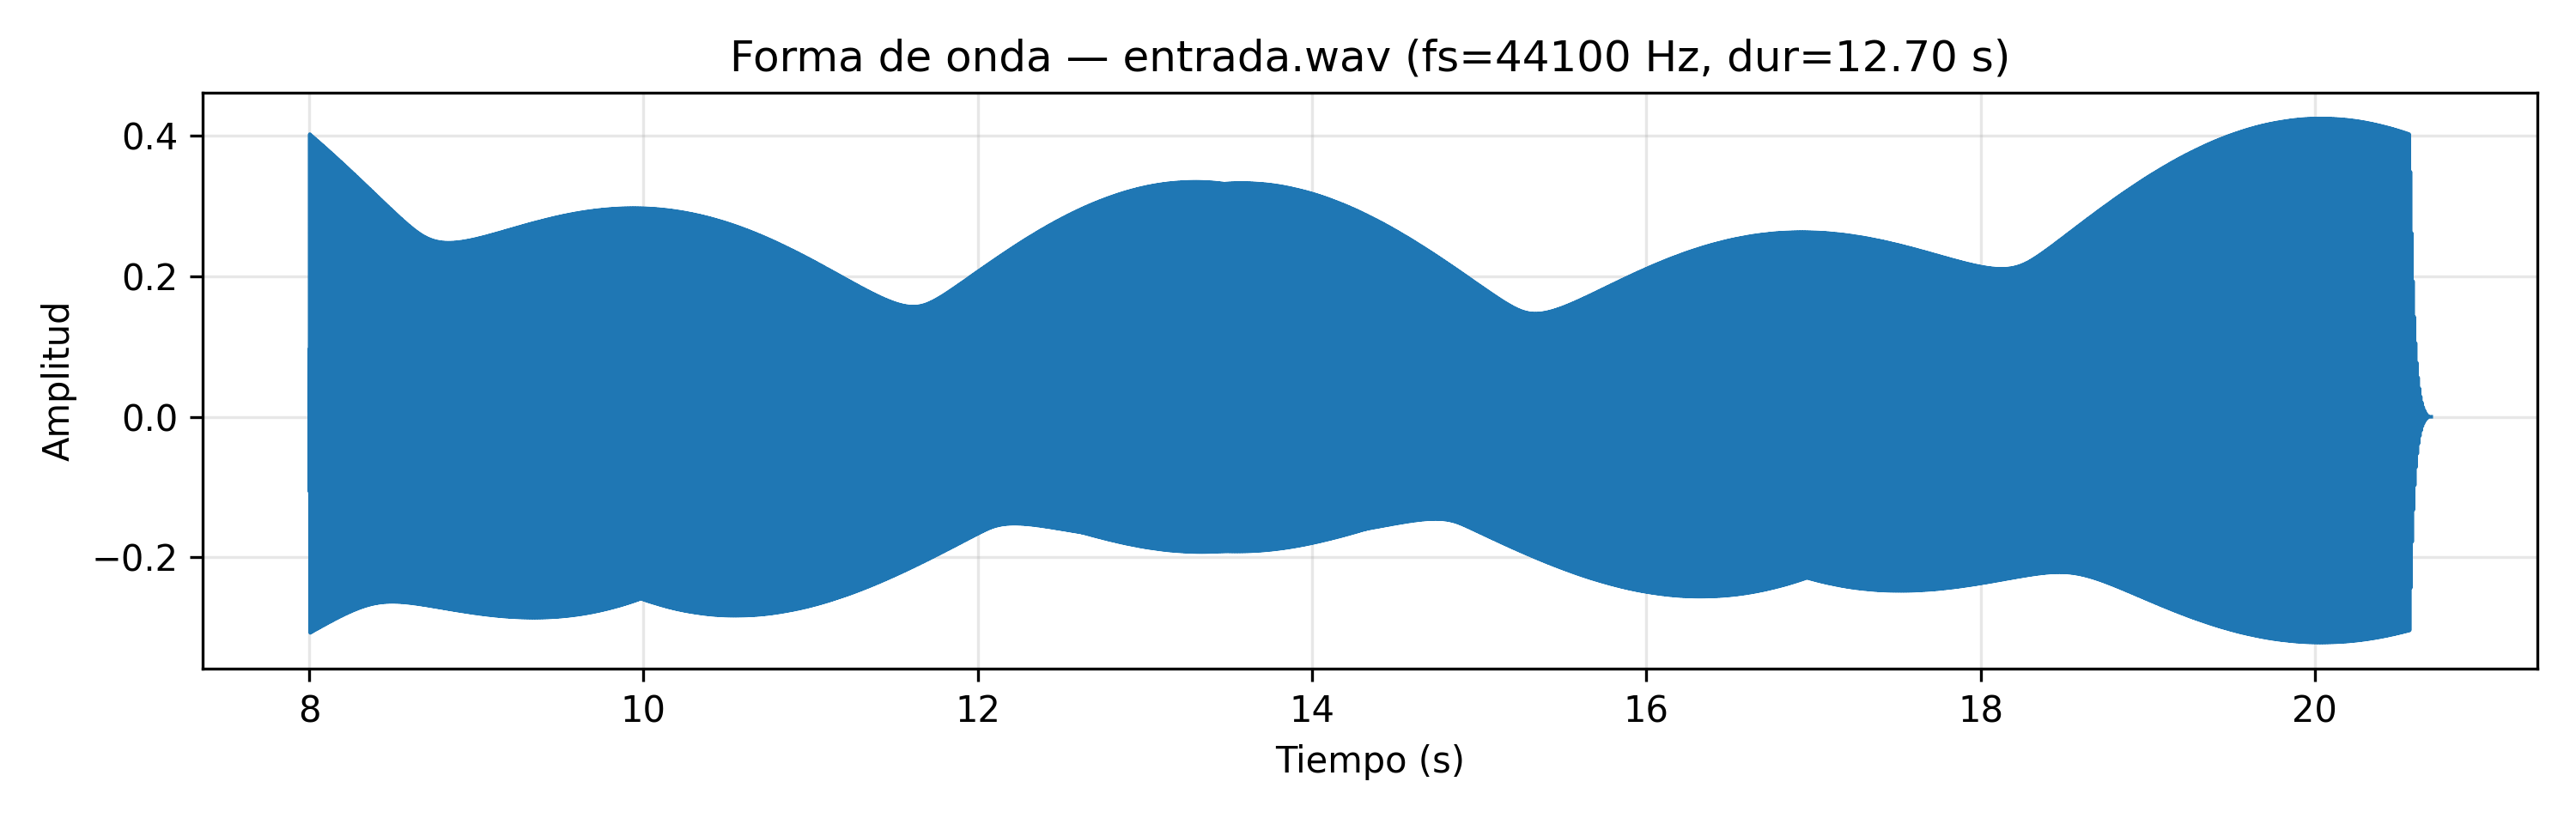
\includegraphics[width=0.98\linewidth]{Media/Figura1.png}
  \caption{Forma de onda del segmento analizado con \(f_s=44.1\) kHz. Se observa una envolvente de batido producida por dos componentes senoidales muy cercanas en frecuencia. El fenómeno temporal es consistente con la separación en frecuencia que se confirma en el dominio espectral.}
  \label{fig:exp1-waveform}
\end{figure}

En la Figura~\ref{fig:exp1-mag-full} se observa un pico dominante alrededor de \(261\) Hz y componentes en \(\sim131\) Hz y \(\sim524\) Hz, consistentes con relación de octavas del material analizado. La energía fuera de esas vecindades cae de forma marcada gracias al uso de ventana de Hann, que atenúa la fuga espectral al reducir los lóbulos laterales respecto de una ventana rectangular, aunque a costa de un lóbulo principal algo más ancho \cite{Harris1978Windows,OppenheimSchaferDTSP3e}. El tamaño base \(N_{\text{base}}=912{,}712\) con \(f_s=44{,}100\) Hz fija una resolución física \(\Delta f \approx 0.0483\) Hz, suficiente para evidenciar la estrechez tonal global sin confundirla con el ruido de fondo numérico \cite{OppenheimSchaferDTSP3e,VetterliKovacevicGoyalFSP2014}.
% ===== Figura 2 =====
\begin{figure}[H]
  \centering
  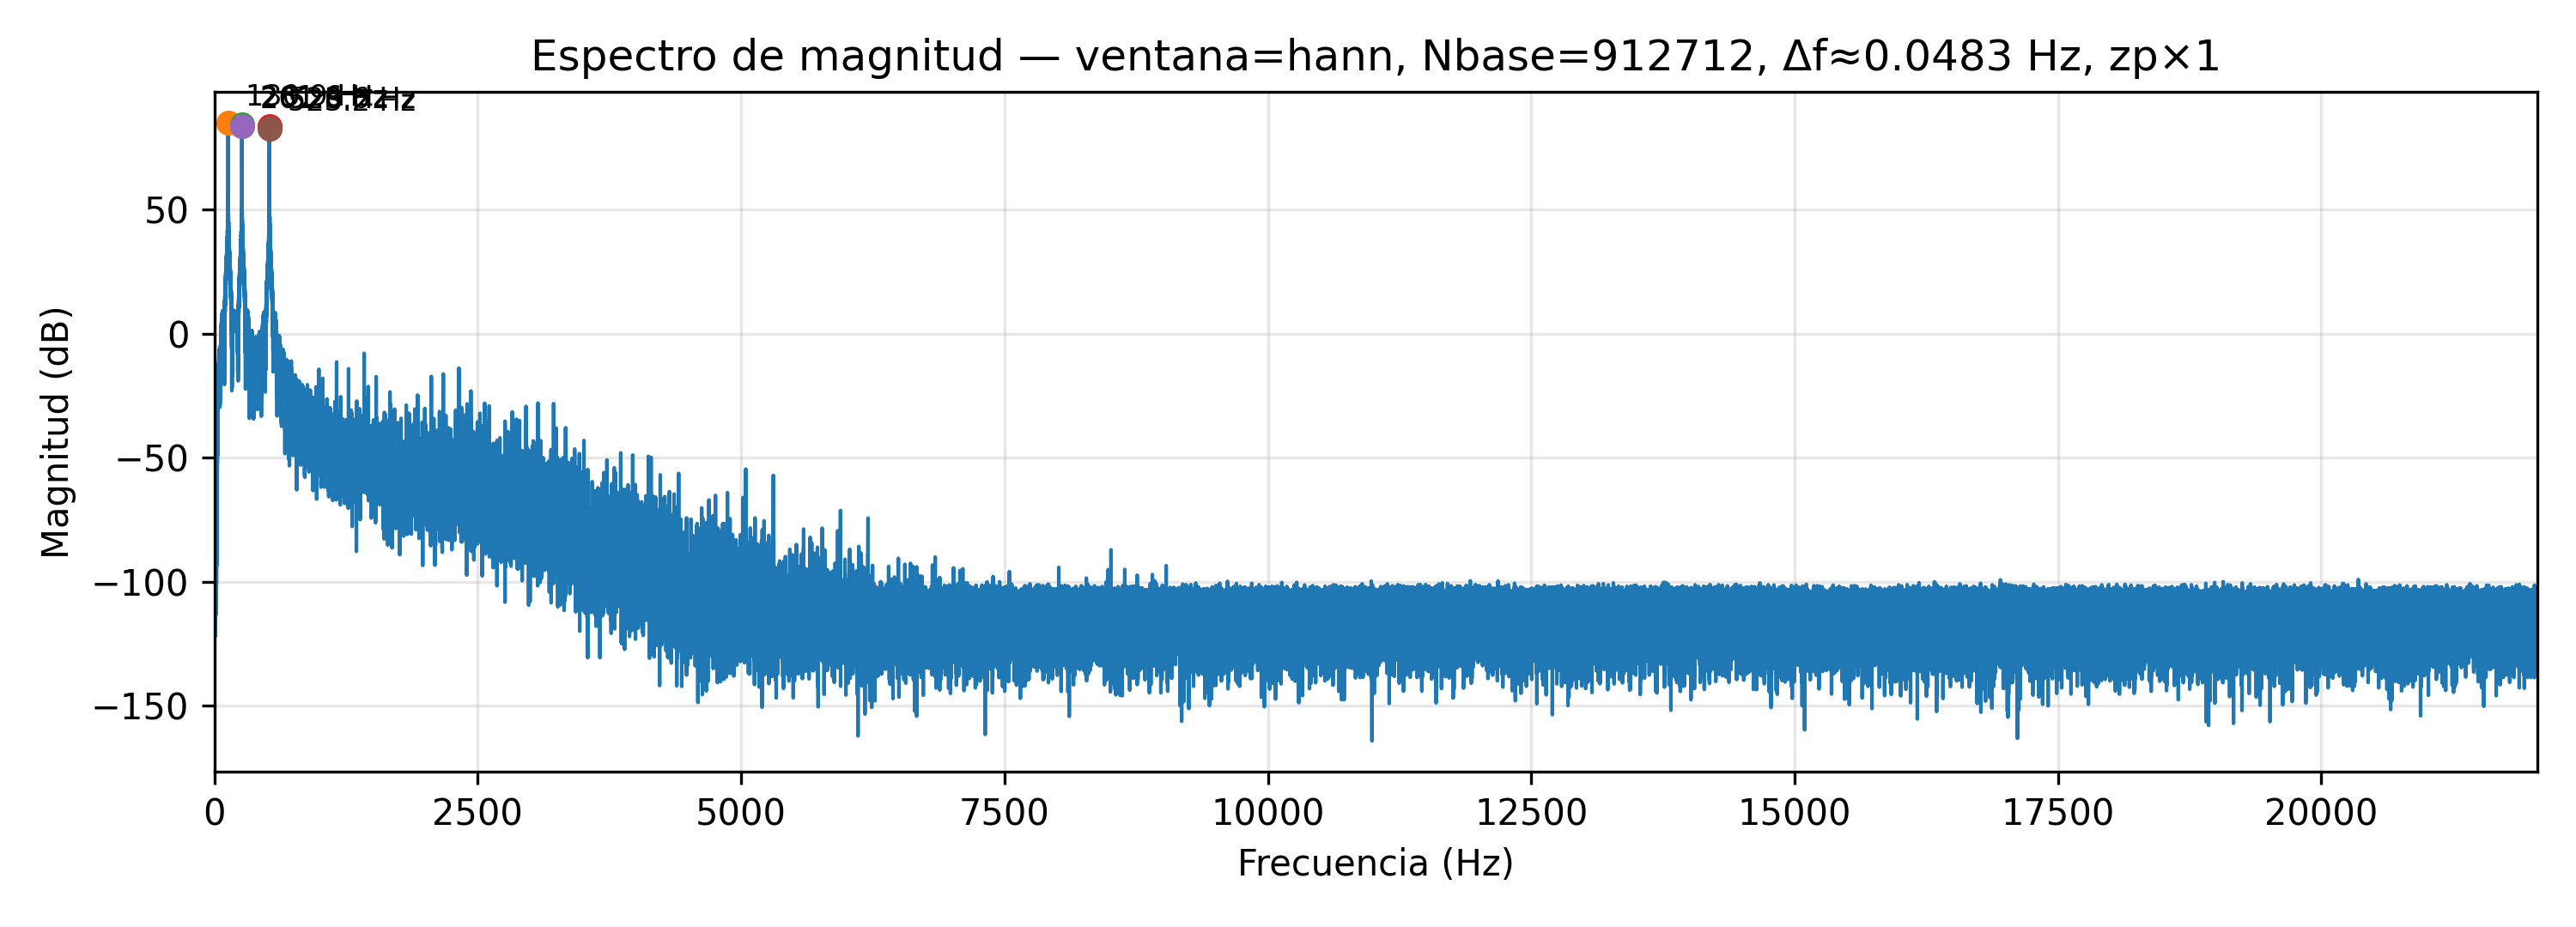
\includegraphics[width=0.98\linewidth]{Media/Figura2.png}
  \caption{Espectro de magnitud en banda completa \((0\)–\(f_s/2)\) con ventana de Hann. Se distinguen la fundamental alrededor de \(261\) Hz y octavas cercanas a \(131\) Hz y \(524\) Hz. El ventaneado reduce la fuga espectral y permite identificar los picos principales.}
  \label{fig:exp1-mag-full}
\end{figure}

La Figura~\ref{fig:exp1-mag-mid} permite distinguir el lóbulo principal de la ventana en torno a la fundamental y la estructura de lóbulos laterales. Con Hann, el primer lóbulo lateral aparece notablemente atenuado y decrece, lo que explica que el espectro fuera de la vecindad tonal permanezca bajo y estable \cite{Harris1978Windows}. El ensanchamiento del lóbulo principal observado es el comportamiento esperado de una transformada de duración finita: cuanto mayor sea \(N_{\text{base}}\), más estrecho resultará el lóbulo y mejor la separabilidad de componentes cercanas \cite{OppenheimSchaferDTSP3e}. 
% ===== Figura 3 =====
\begin{figure}[H]
  \centering
  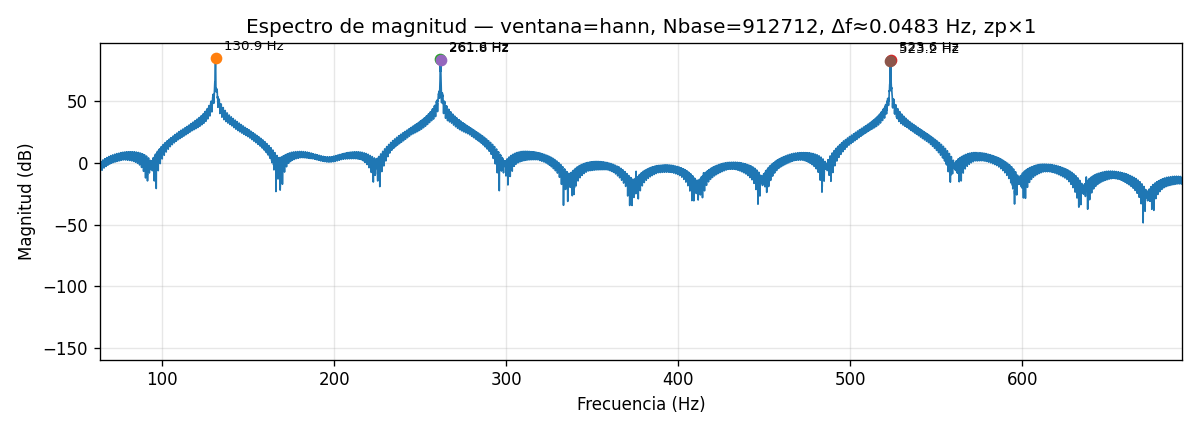
\includegraphics[width=0.98\linewidth]{Media/Figura3.png}
  \caption{Espectro de magnitud con zoom intermedio \((60\)–\(650\) Hz). Se aprecia con mayor detalle la zona tonal y los lóbulos laterales asociados al uso de la ventana de Hann.}
  \label{fig:exp1-mag-mid}
\end{figure}

En la Figura \ref{fig:exp1-mag-zoom} se resolvió el doblete alrededor de \(261\) Hz. En la corrida mostrada, la consola reportó picos en \(f\approx 261.6\) Hz y \(f\approx 261.8\) Hz, con una separación \(\Delta f\) medida del orden de \(0.15\)–\(0.20\) Hz. Esta separación concuerda con la predicción para un intervalo de un cent alrededor de \(f_0\) (\(\Delta f_{\text{cent}} \approx f_0(2^{1/1200}-1)\)), que para \(f_0\approx 261\) Hz vale $\approx$ \(0.15\) Hz \cite{OsgoodFTAMS2019}. La capacidad de distinguir ambas líneas está limitada por la resolución física \(\Delta f=f_s/N_{\text{base}}\); el \emph{zero padding} solo densifica la rejilla de muestreo frecuencial y mejora la lectura, pero no reduce el ancho efectivo del lóbulo ni aumenta la verdadera resolución \cite{OppenheimSchaferDTSP3e,Harris1978Windows}.

% ===== Figura 4 =====
\begin{figure}[H]
  \centering
  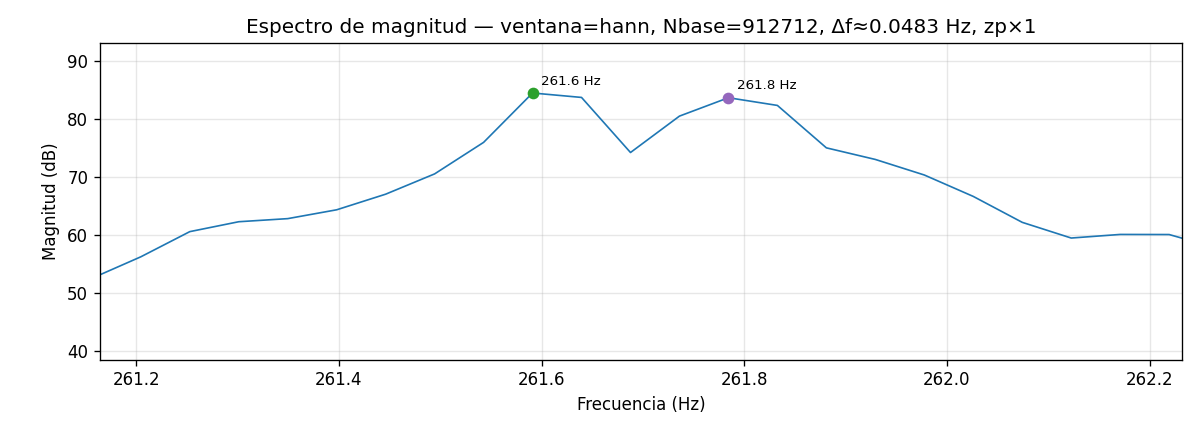
\includegraphics[width=0.98\linewidth]{Media/Figura4.png}
  \caption{Espectro de magnitud con zoom alrededor de \(261\) Hz. Se observan dos picos muy cercanos (por ejemplo, \(261.6\) Hz y \(261.8\) Hz), con separación aproximada de \(0.15\)–\(0.20\) Hz, coherente con un intervalo de un cent. El \emph{zero padding} densifica la rejilla de lectura, pero la resolución física viene dada por \(\Delta f=f_s/N_{\text{base}}\).}
  \label{fig:exp1-mag-zoom}
\end{figure}

La Figura~\ref{fig:exp1-phase} exhibe una pendiente global aproximadamente lineal de la fase con la frecuencia. Este comportamiento es característico de un desplazamiento temporal del segmento analizado: un corrimiento en tiempo introduce una rotación lineal de fase en el dominio de la frecuencia \cite{OppenheimSchaferDTSP3e,VetterliKovacevicGoyalFSP2014}. Al hacer zoom en la vecindad de las líneas alrededor de \(261\) Hz, la fase desenrollada se mantiene suave y coherente con componentes casi sinusoidales; las variaciones abruptas alejadas de las líneas se asocian a bajo nivel de señal y a los efectos del ventaneo \cite{OppenheimSchaferDTSP3e}.
% ===== Figura 5 =====
\begin{figure}[H]
  \centering
  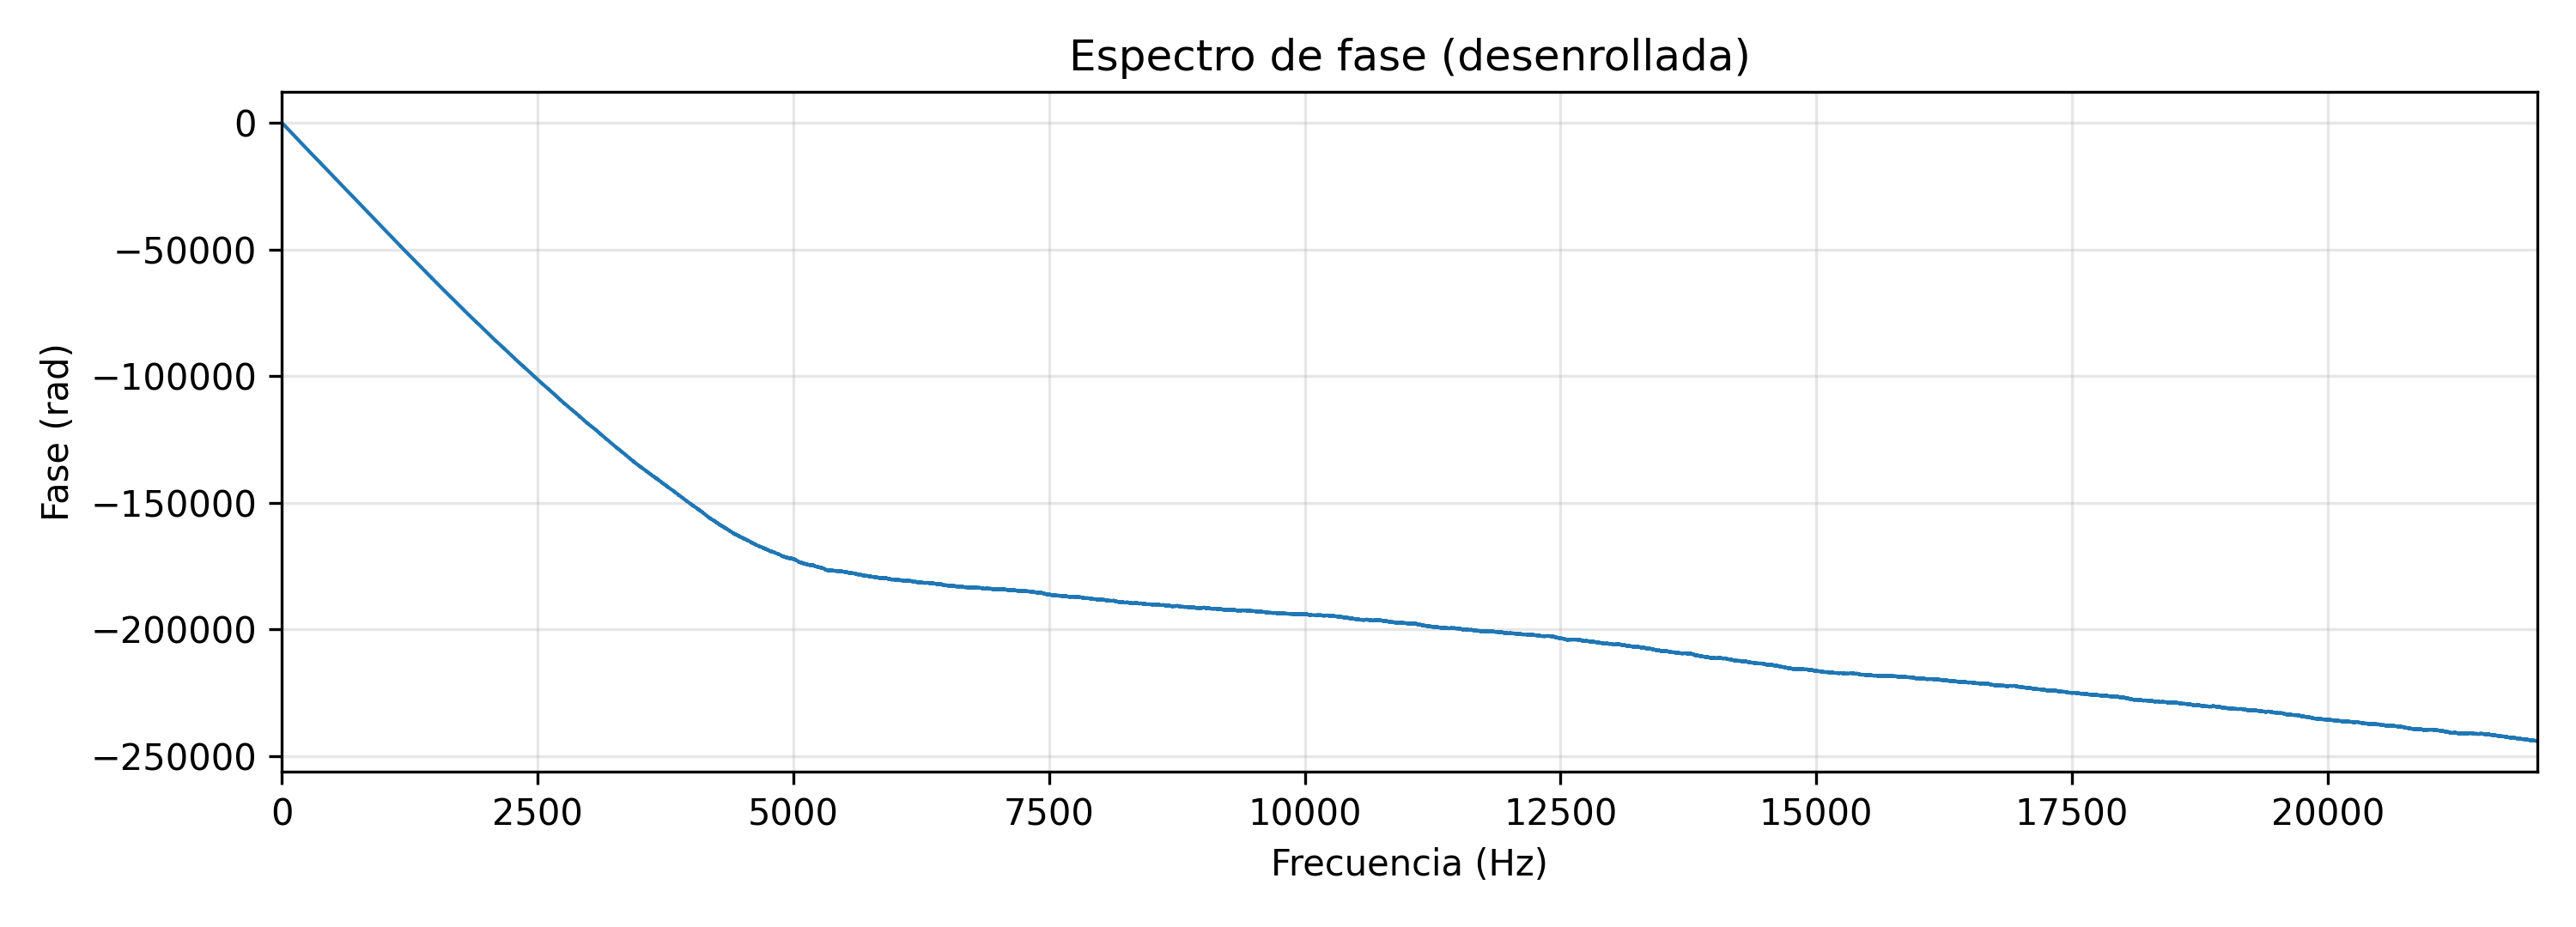
\includegraphics[width=0.98\linewidth]{Media/Figura5.png}
  \caption{Espectro de fase desenrollada. A escala ancha aparece una pendiente global asociada al origen temporal del segmento; localmente, en torno a las líneas de \(261\) Hz, la fase muestra un comportamiento suave característico de tonos casi puros.}
  \label{fig:exp1-phase}
\end{figure}  

En conjunto, los resultados confirman la relación tiempo–frecuencia esperada: la envolvente de batido en el dominio temporal y el doblete en el dominio frecuencial son dos manifestaciones del mismo fenómeno físico-matemático. La configuración empleada (Hann, \(N_{\text{base}}=912{,}712\), \(\Delta f=0.0483\) Hz) resulta suficiente para identificar el par de líneas cercanas, y la lectura es consistente con el intervalo de un cent alrededor de \(261\) Hz \cite{OppenheimSchaferDTSP3e,Harris1978Windows}.



% =========================
\section{Uso de Fourier en modulación y demodulación}

\subsection{Diagrama de bloques del sistema}

% --- Añadir imágenes de modulación y desmodulación FSK ---
\begin{figure}[H]
  \centering
  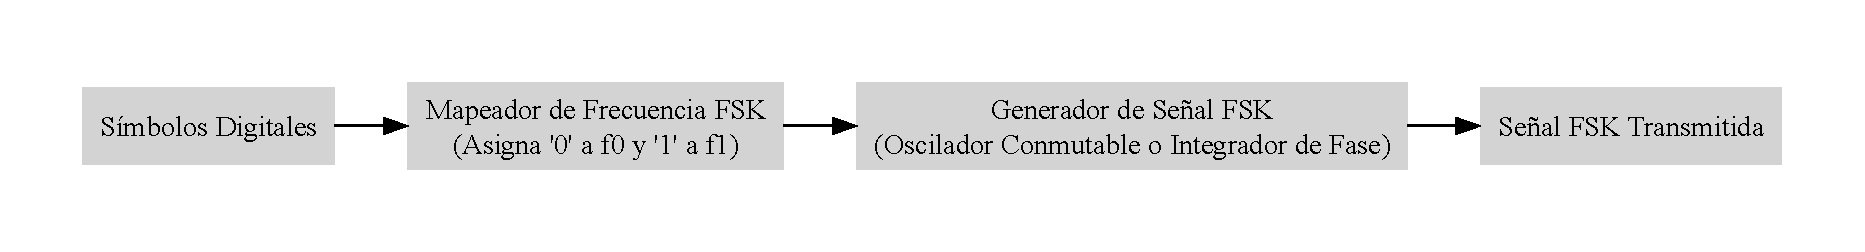
\includegraphics[width=0.95\linewidth]{diagrama_fsk_mod.pdf}
  \caption{Diagrama de bloques del sistema de modulación FSK.}
  \label{fig:bloques-mod-fsk}
\end{figure}

\begin{figure}[H]
  \centering
  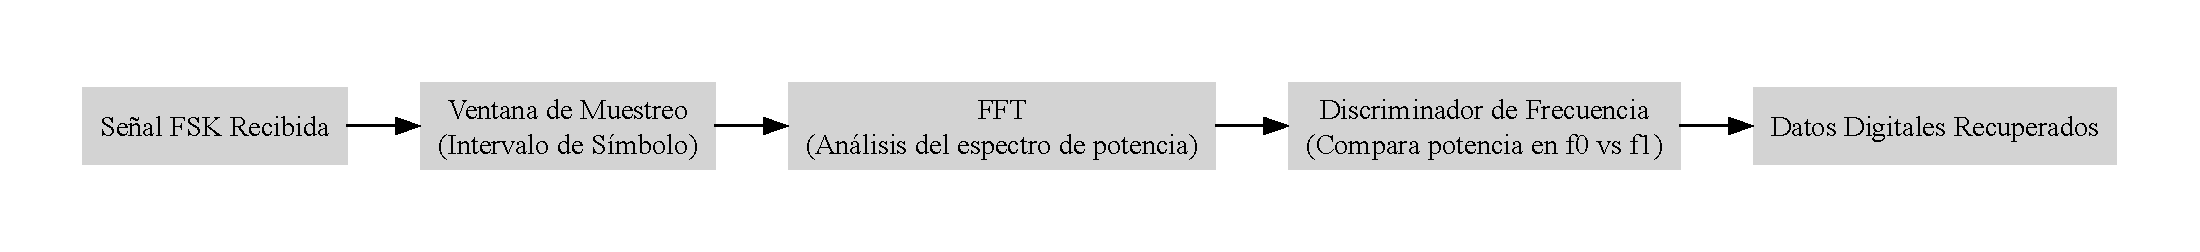
\includegraphics[width=0.95\linewidth]{diagrama_fsk_desmod.pdf}
  \caption{Diagrama de bloques del sistema de desmodulación FSK.}
  \label{fig:bloques-desmod-fsk}
\end{figure}

La modulación FSK (Frequency Shift Keying) utiliza la transformada de Fourier (FT) para el análisis espectral de la señal, que permite verificar cómo la energía de la señal se distribuye a través de las frecuencias de transmisión. En este contexto, la Transformada Rápida de Fourier (FFT) se aplica tanto en la modulación como en la demodulación para asegurar una correcta transmisión y recuperación de la señal \cite{McCune2010}.

El diagrama de bloques del sistema de modulación-demodulación FSK se muestra a continuación. En este sistema, la señal de datos binarios es modulada en función de las frecuencias \( f_0 \) y \( f_1 \), que representan los bits '0' y '1', respectivamente \cite{McCune2010}.

\begin{figure}[H]
  \centering
  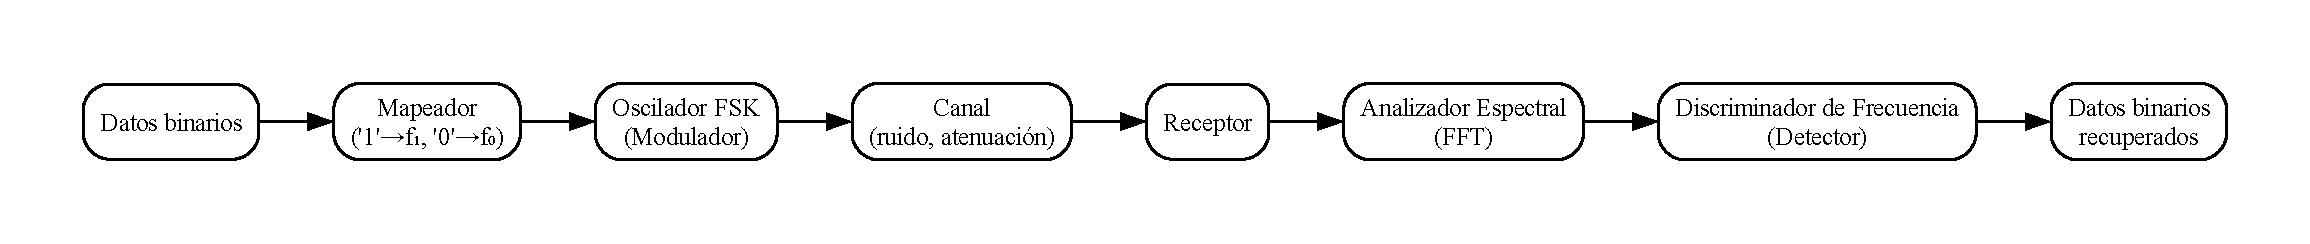
\includegraphics[width=0.95\linewidth]{diagrama_mod_demod_fsk.pdf} % <-- reemplaza con tu diagrama
  \caption{Diagrama de bloques del modulador-demodulador considerado.}
  \label{fig:bloques-mod-demod}
\end{figure}

\subsubsection{Señales esperadas en cada bloque}
Al aplicar la FT o la FFT en cada bloque del sistema, podemos observar cómo se distribuyen las señales en el dominio de la frecuencia. Las señales baseband (de banda base), las portadoras y las bandas laterales varían según el tipo de modulación. Además, se identifican los puntos donde ocurre la traslación de frecuencia y el filtrado \cite{McCune2010}.

\subsection{Lectura en el dominio de Fourier}

En esta sección, se explica cómo se verían las señales en el dominio de Fourier a lo largo del proceso de modulación y demodulación FSK \cite{McCune2010}.

\subsubsection{1. Uso de la Transformada de Fourier (FT/FFT) en FSK}

La modulación FSK varía la frecuencia de la portadora de acuerdo con los símbolos transmitidos: \( f_0 \) para el bit 0 y \( f_1 \) para el bit 1. El uso de la FT (o más comúnmente la FFT en sistemas digitales) es esencial para el análisis espectral de la señal y para verificar que la energía de la señal esté distribuida correctamente en el dominio de la frecuencia \cite{McCune2010}.

\paragraph{A. En la Modulación FSK}

Aunque la FT/FFT no es parte directa de la generación de la señal FSK, sí es crucial para el análisis y diseño del sistema de modulación:

\begin{itemize}
    \item \textbf{Verificación Espectral:} Al aplicar la FFT a la señal modulada FSK \( s(t) \), se obtiene su Densidad Espectral de Potencia (PSD), lo que permite observar cómo se distribuye la energía de la señal a lo largo de las frecuencias \( f_0 \) y \( f_1 \). La FFT asegura que la energía se concentre correctamente en las frecuencias de señalización\cite{McCune2010}.
    \item \textbf{Control del Ancho de Banda:} Aunque el ancho de banda de una señal FSK es teóricamente infinito, la FFT permite observar que, en la práctica, la señal tiene una PSD acotada. Esto es importante para asegurar que la señal se ajuste al ancho de banda asignado, lo que es crucial para evitar interferencias y cumplir con las restricciones del canal de comunicación\cite{McCune2010}.
\end{itemize}

\paragraph{B. En la Demodulación FSK}

El objetivo principal de la demodulación FSK es determinar, a partir de la señal recibida \( r(t) \), cuál de los símbolos \( m_0 \) o \( m_1 \) se ha transmitido. Este proceso se realiza utilizando la FFT para analizar el contenido de frecuencia de la señal recibida\cite{McCune2010}.

\begin{table}[H]
\centering
\begin{tabularx}{0.98\linewidth}{|l|X|}
\hline
\textbf{Bloque de Demodulación (Funcional)} & \textbf{Uso de la FFT} \\ \hline
Receptor de la Señal  & Recibe la señal FSK \( r(t) \), la cual puede estar afectada por ruido y atenuación. \\ \hline
Analizador Espectral (FFT) & La FFT se aplica a la señal \( r(t) \) en cada intervalo de símbolo \( T_S \), permitiendo determinar las frecuencias dominantes (espectro de la señal). \\ \hline
Discriminador de Frecuencia/Detector & Utiliza la información de la FFT para comparar la energía en las ubicaciones de \( f_0 \) y \( f_1 \), y determina el símbolo transmitido. La frecuencia con el mayor pico de magnitud o potencia es la que corresponde al símbolo original ('0' o '1'). \\ \hline
\end{tabularx}
\caption{Tabla de bloques en el proceso de demodulación FSK y su relación con la FFT.}
\end{table}

\subsubsection{2. Diagrama de Bloques Conceptual de Modulación FSK}

La modulación FSK implica conmutar entre dos (o más) frecuencias portadoras distintas, basándose en el símbolo entrante. El proceso de modulación FSK es el siguiente:

\begin{itemize}
    \item \textbf{Bloque de Símbolos Digitales:} Recibe una secuencia de datos binarios, por ejemplo, '1', '0', '1', '0'.
    \item \textbf{Bloque de Asignación de Frecuencia:} Mapea '1' a \( f_1 \) y '0' a \( f_0 \).
    \item \textbf{Bloque de Osciladores FSK:} Genera la señal \( s(t) \) modulada, con las frecuencias portadoras \( f_0 \) y \( f_1 \).
\end{itemize}

El proceso se ve de la siguiente manera:

$$ \mathbf{Datos\ Binarios} \longrightarrow \mathbf{Mapeador\ } ('1' \to f_1, '0' \to f_0) \longrightarrow \mathbf{Oscilador\ de\ FSK} \longrightarrow \mathbf{s(t)} $$

\subsubsection{3. Observación de las Señales en el Dominio de la Frecuencia}

Al aplicar la FFT a una señal FSK, se obtiene el Espectro de Potencia (PSD). Este espectro muestra los picos de energía en las frecuencias \( f_0 \) y \( f_1 \). Para una señal 2-FSK (binaria), el espectro se observa de la siguiente manera:

\begin{itemize}
    \item \textbf{Picos de Frecuencia Positiva:} Se observan dos picos de frecuencia, uno a \( f_0 \) y otro a \( f_1 \), que corresponden a los bits '0' y '1', respectivamente.
    \item \textbf{Frecuencia Portadora:} El espectro puede estar centrado alrededor de una frecuencia portadora \( f_c \), que se encuentra en el centro de los picos \( f_0 \) y \( f_1 \).
\end{itemize}
  
El índice de modulación \( h \) determina la distancia entre los picos de frecuencia, que se relaciona con el tiempo de símbolo \( T_S \). Este análisis espectral es crucial para la correcta interpretación de la señal en sistemas FSK.

\subsection{Cómo se observan las señales}

La siguiente figura muestra el ejemplo de modulación FSK para la secuencia binaria 10101. Se presentan tres gráficas: la señal de datos, las portadoras asociadas a cada bit y la señal modulada resultante \cite{Ktims2006}.

\begin{figure}[H]
  \centering
  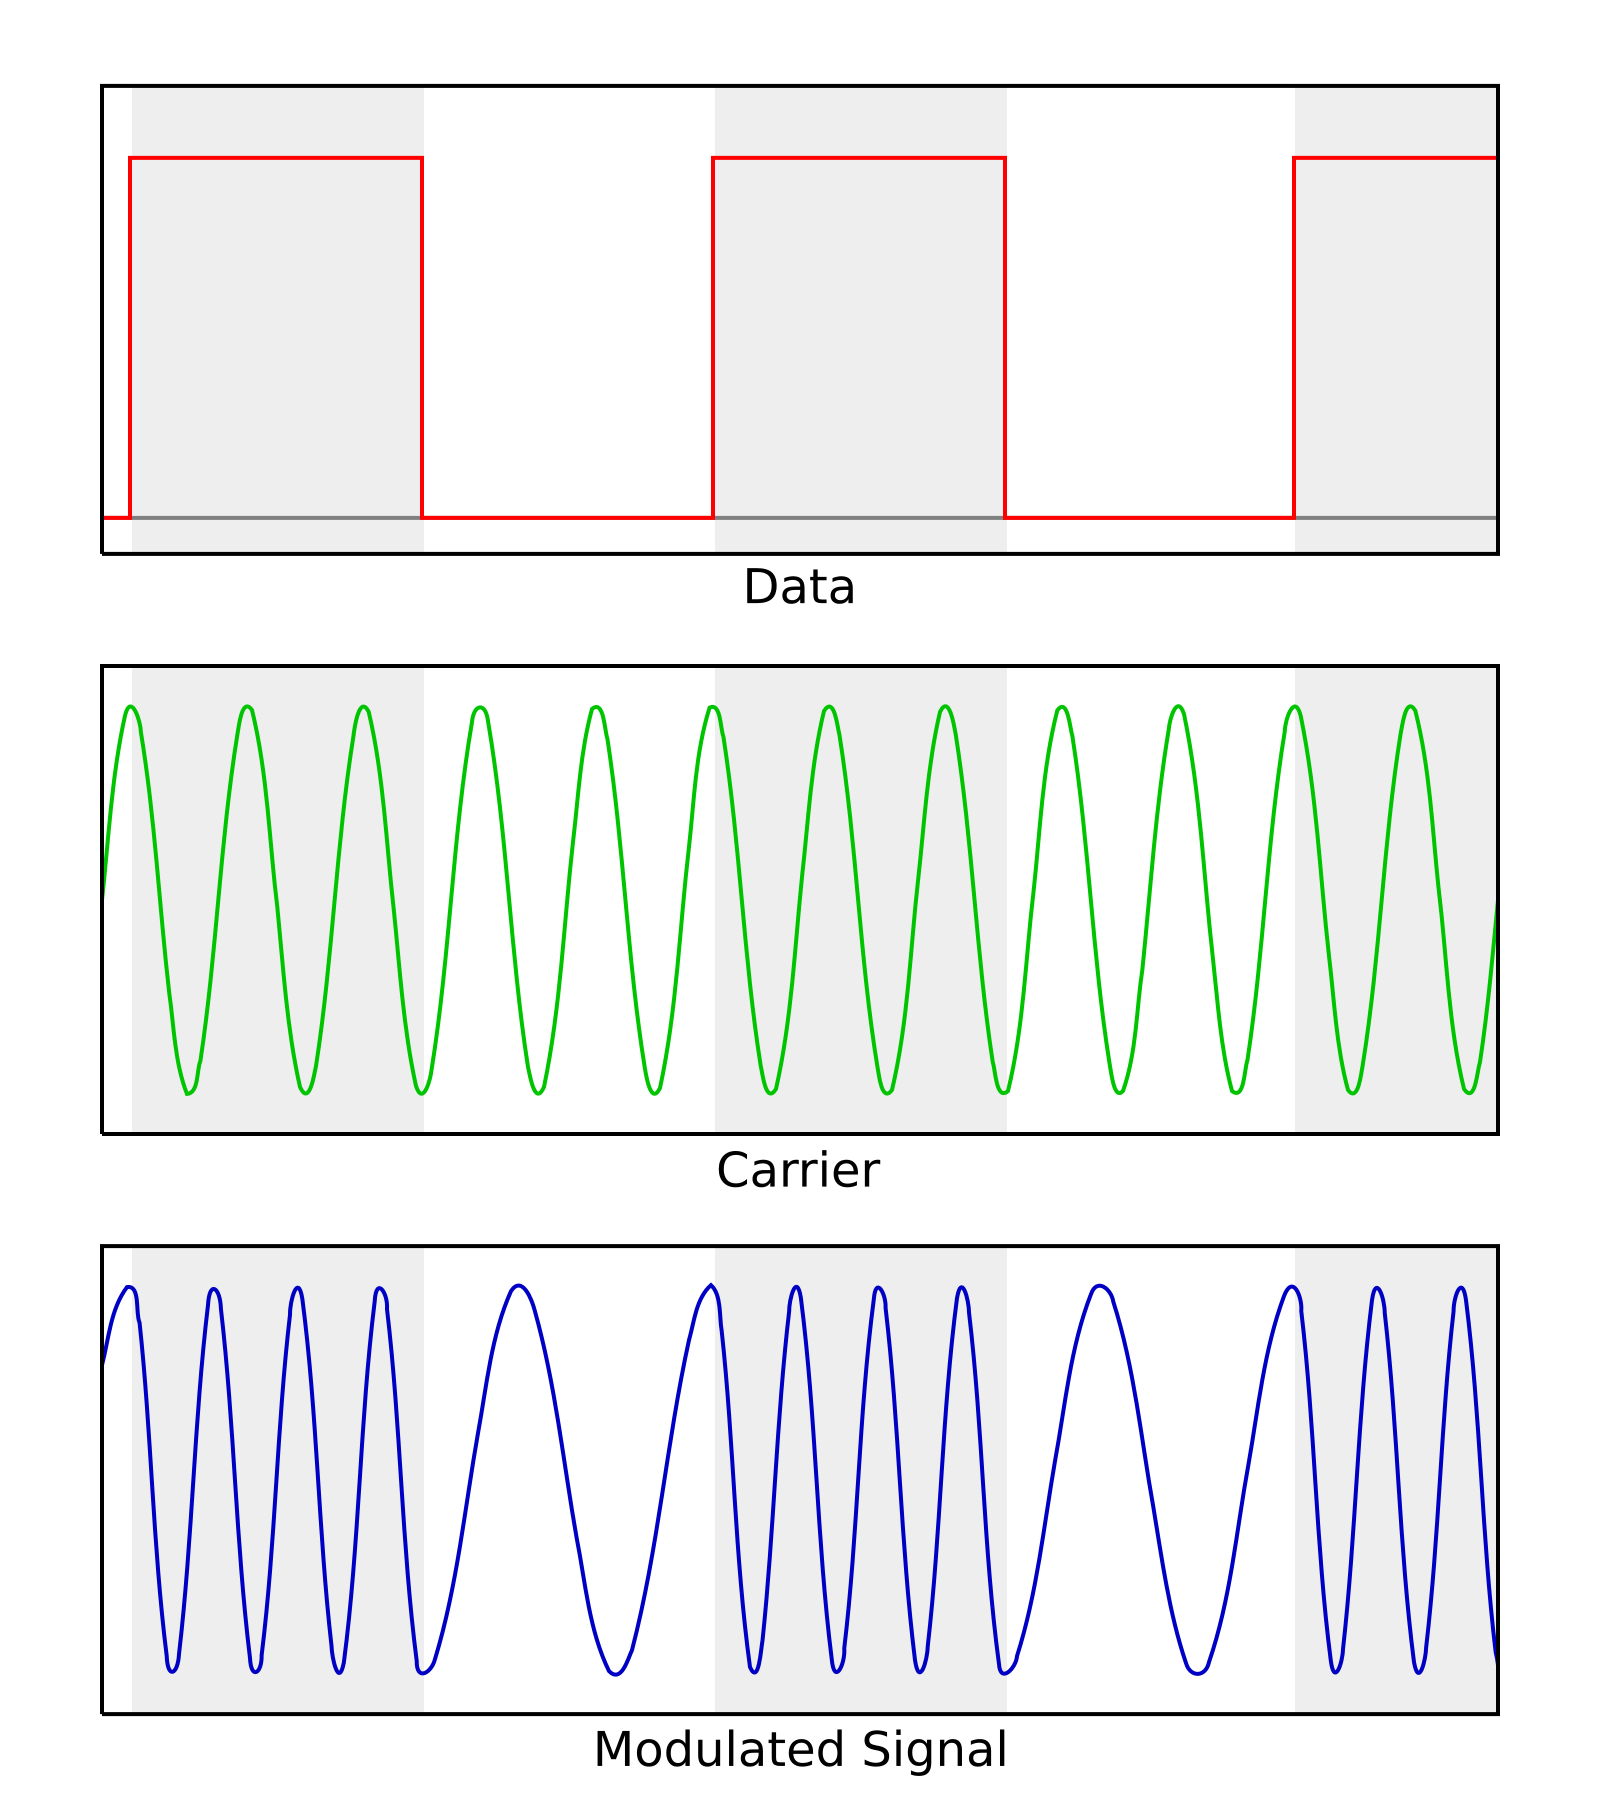
\includegraphics[width=0.5\linewidth]{Media/Fsk.svg.png}
  \caption{Ejemplo de modulación FSK para la secuencia binaria 10101. Arriba: señal de datos; medio: portadoras para cada bit; abajo: señal modulada FSK. \cite{Ktims2006}}
  \label{fig:fsk-ejemplo}
\end{figure}

% =========================
\section{Bibliotecas y \emph{drivers} en microcontroladores}

\subsection{Biblioteca/Driver}

A continuación se resumen las bibliotecas y drivers relevantes para implementar un sistema FSK en microcontroladores:

\begin{longtable}{|p{2.5cm}|p{3cm}|p{4cm}|p{5cm}|}
\hline
\textbf{Bloque} & \textbf{MCU  Firmware} & \textbf{Driver Bibliotecas} & \textbf{Descripción} \\ \hline
Modulador FSK & ARM Cortex & CMSIS-DSP \Cite{Condes2024_CMSIS_DSP} & Generación eficiente de señales FSK y operaciones matemáticas. \\ \hline
Modulador FSK & Arduino & Arduino FFT Library \Cite{ArduinoFFT_docs} & Procesamiento de señales y FFT en plataformas Arduino. \\ \hline
Modulador FSK & PC/Simulación & MATLAB/Simulink & Simulación y prototipado previo a implementación en hardware. \\ \hline
Canal de comunicación & MCU genérico & SPI & Transmisión rápida de datos binarios entre dispositivos. \\ \hline
Canal de comunicación & MCU genérico & I2C & Comunicación sencilla y con pocos cables entre dispositivos. \\ \hline
Demodulador FSK & ARM Cortex & CMSIS-DSP \Cite{Condes2024_CMSIS_DSP}& FFT eficiente para análisis de señales recibidas. \\ \hline
Demodulador FSK & Arduino & Arduino FFT Library \Cite{ArduinoFFT_docs} & Análisis de frecuencia en señales recibidas. \\ \hline
Demodulador FSK & Microchip PIC32 & MPLAB Harmony \Cite{Microchip_MPLAB_Harmony}& Procesamiento avanzado de señales y FFT. \\ \hline
Demodulador FSK & TI DSP & TI DSP Libraries \Cite{TI_MSPDSPLIB} & Funciones optimizadas para FFT en DSPs de Texas Instruments. \\ \hline
\end{longtable}

\vspace{0.5em}
\noindent\textbf{Tabla:} Bibliotecas y drivers relevantes para modulación/demodulación FSK en microcontroladores.

% =========================
% ...existing code...
\section{Prototipo en PC: modulación y demodulación}
% Esta sección cubre la parte 5 (demo PC). Solo resultados e interpretación.
\subsection{Especificación del esquema de modulación}
Se implementó un esquema 2-FSK (binary FSK) sin canal ruidoso:
\begin{itemize}
  \item Frecuencia de muestreo: \(f_s = 44{,}100\) Hz (corrida base de exp5.py).
  \item Duración de símbolo: \(T_b = 0.1\) s \(\Rightarrow N_s = f_s T_b = 4410\) muestras/símbolo.
  \item Frecuencias de señalización: \(f_0 = 1000\) Hz (bit 0), \(f_1 = 2000\) Hz (bit 1).
  \item Amplitud: \(A=0.8\) (señal normalizada a \([-1,1]\) al guardar WAV).
  \item FFT por símbolo (demod): ventana Hann, factor de \emph{zero padding} \(zp=2\) (malla más densa), magnitud en dB.
  \item Resolución frecuencial efectiva por símbolo: \(\Delta f \approx \frac{f_s}{N_s} \approx 10\) Hz.
\end{itemize}
Además, para ilustración visual se generaron figuras complementarias con \(f_s=10\) kHz y \(T_b=1\) s (archivos fsk\_demo\_*.png), sin afectar los resultados de BER.

\subsubsection{Procedimiento experimental}
\begin{enumerate}
  \item TX: generación de bits (patrón por defecto ``1011010''), mapeo \(0\to f_0\), \(1\to f_1\), concatenación de tonos seno por símbolo.
  \item Se guarda el audio en WAV y se grafica la onda completa.
  \item RX: para cada símbolo \([iT_b,(i+1)T_b]\), se calcula la FFT con ventana Hann y se toma el pico dominante; se decide \(b_i=\arg\min\{|f_{\text{pico}}-f_0|,|f_{\text{pico}}-f_1|\}\).
  \item Se reporta BER y se guardan figuras por símbolo (onda, magnitud dB, fase desenrollada).
\end{enumerate}
Ejecución (desde \texttt{Codigo\_Fuente/}):
\begin{verbatim}
python exp5.py --fs 44100 --Tb 0.1 --f0 1000 --f1 2000 --bits 1011010
\end{verbatim}
Salidas principales en \texttt{Codigo\_Fuente/figs}: 
\texttt{fsk\_waveform.png}, \texttt{fsk\_demo\_overview.png}, 
\texttt{fsk\_demo\_zoom\_spectrogram.png}, 
\texttt{magnitude\_db\_fsk\_bit{i}.png}, 
\texttt{phase\_unwrapped\_fsk\_bit{i}.png}, 
\texttt{waveform\_fsk\_bit{i}.png}.

\subsection{Resultados en el tiempo}
% - Figuras de señal modulada y demodulada en el tiempo. Rotular ejes con unidades.
\begin{figure}[H]
  \centering
  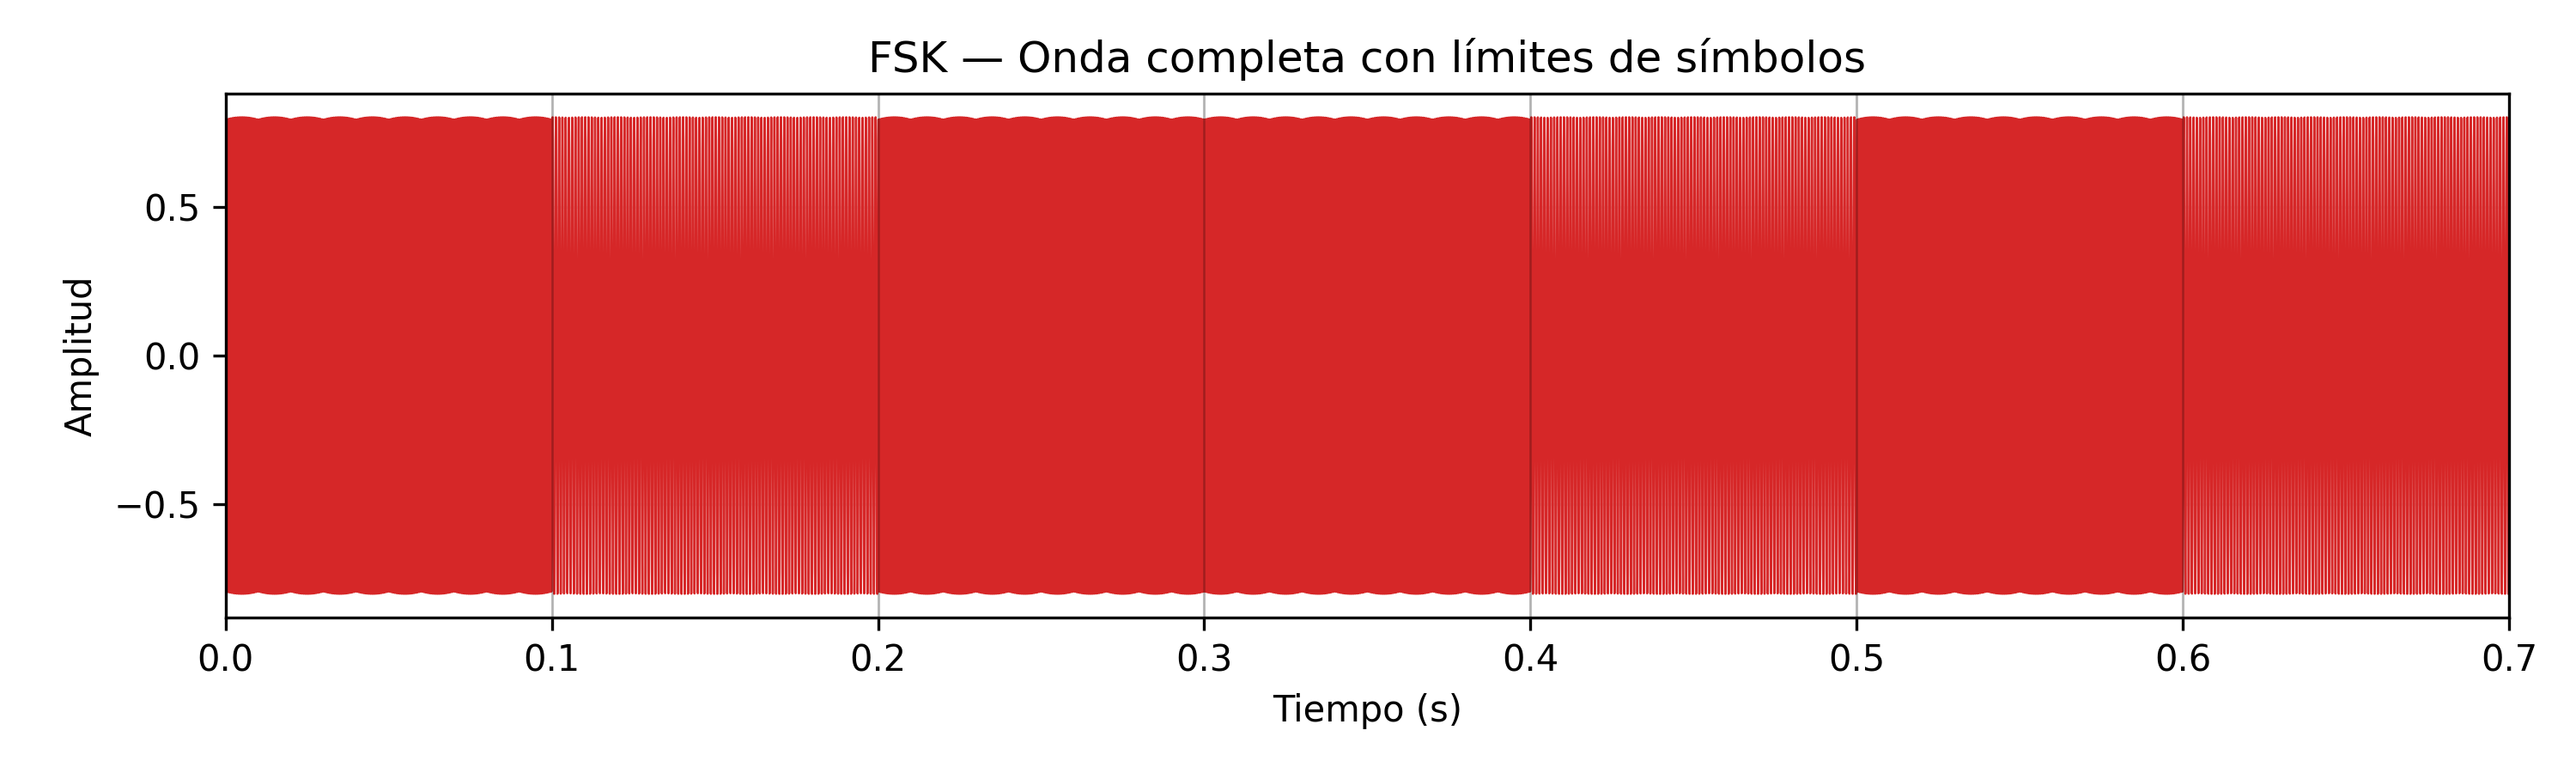
\includegraphics[width=0.95\linewidth]{../Codigo_Fuente/figs/fsk_waveform_full.png}
  \caption{Señal FSK modulada (vista completa). Eje x: tiempo [s]; eje y: amplitud. Las transiciones por símbolo muestran el cambio entre \(f_0\) y \(f_1\).}
  \label{fig:mod-tiempo}
\end{figure}

\begin{figure}[H]
  \centering
  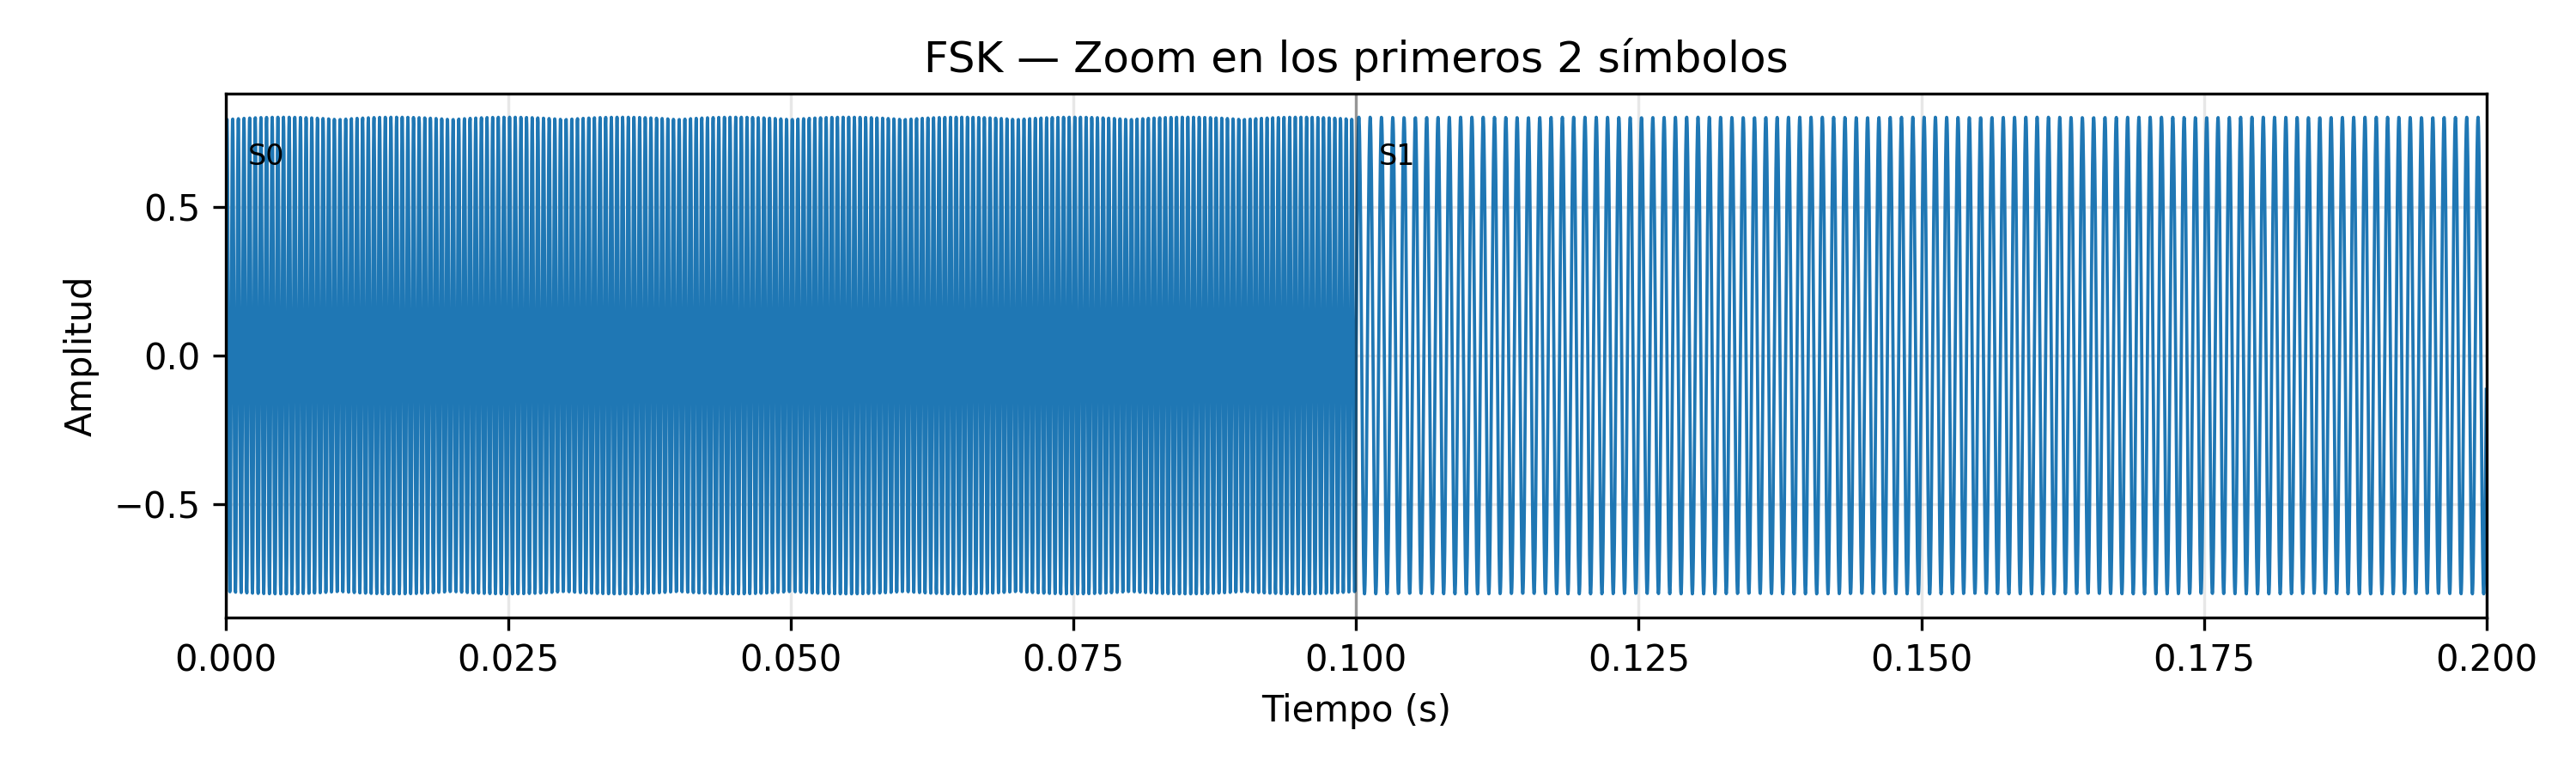
\includegraphics[width=0.95\linewidth]{../Codigo_Fuente/figs/fsk_waveform_zoom.png}
  \caption{Zoom temporal por símbolos. Esta misma segmentación se usa en la demodulación por FFT para estimar el pico de frecuencia por símbolo.}
  \label{fig:demod-tiempo}
\end{figure}

\subsection{Resultados en frecuencia}
% - Espectros de la señal modulada y demodulada (magnitud; opcional fase).
\begin{figure}[H]
  \centering
  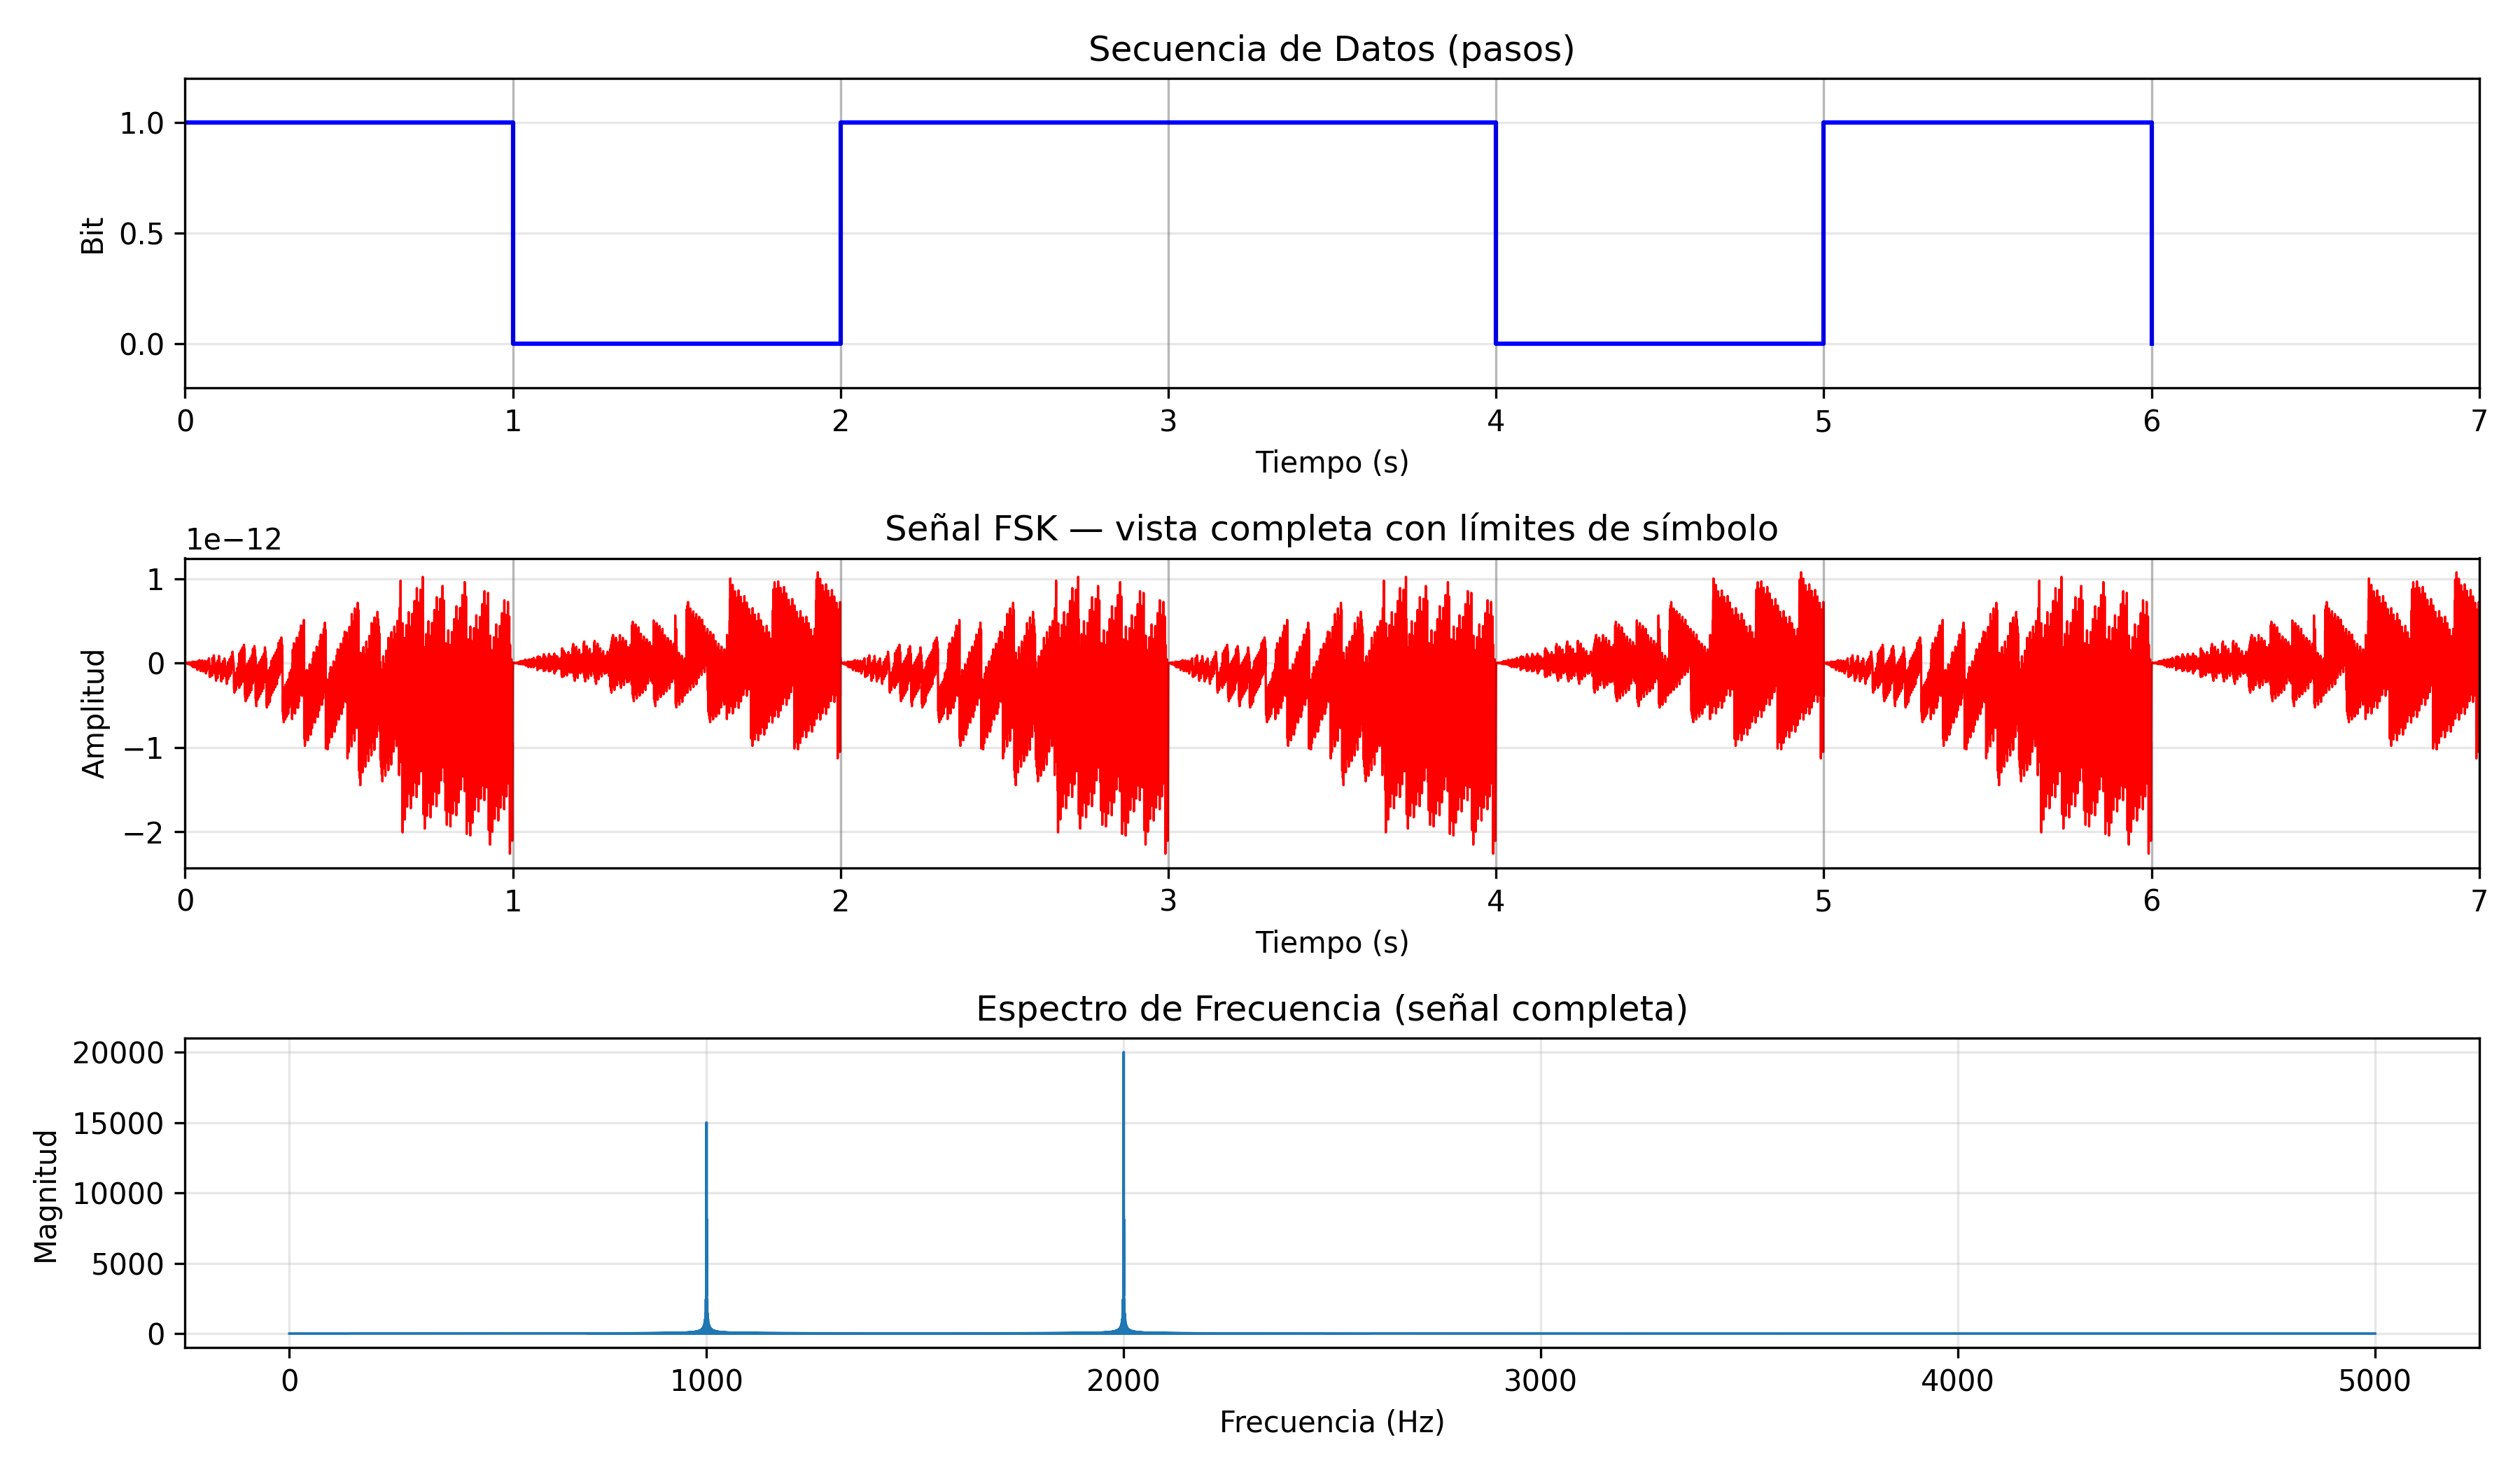
\includegraphics[width=0.95\linewidth]{../Codigo_Fuente/figs/fsk_demo_overview.png}
  \caption{Espectro de la señal FSK completa: picos concentrados en \(f_0\) y \(f_1\). El uso de ventana Hann atenúa lóbulos laterales.}
  \label{fig:mod-freq}
\end{figure}

\begin{figure}[H]
  \centering
  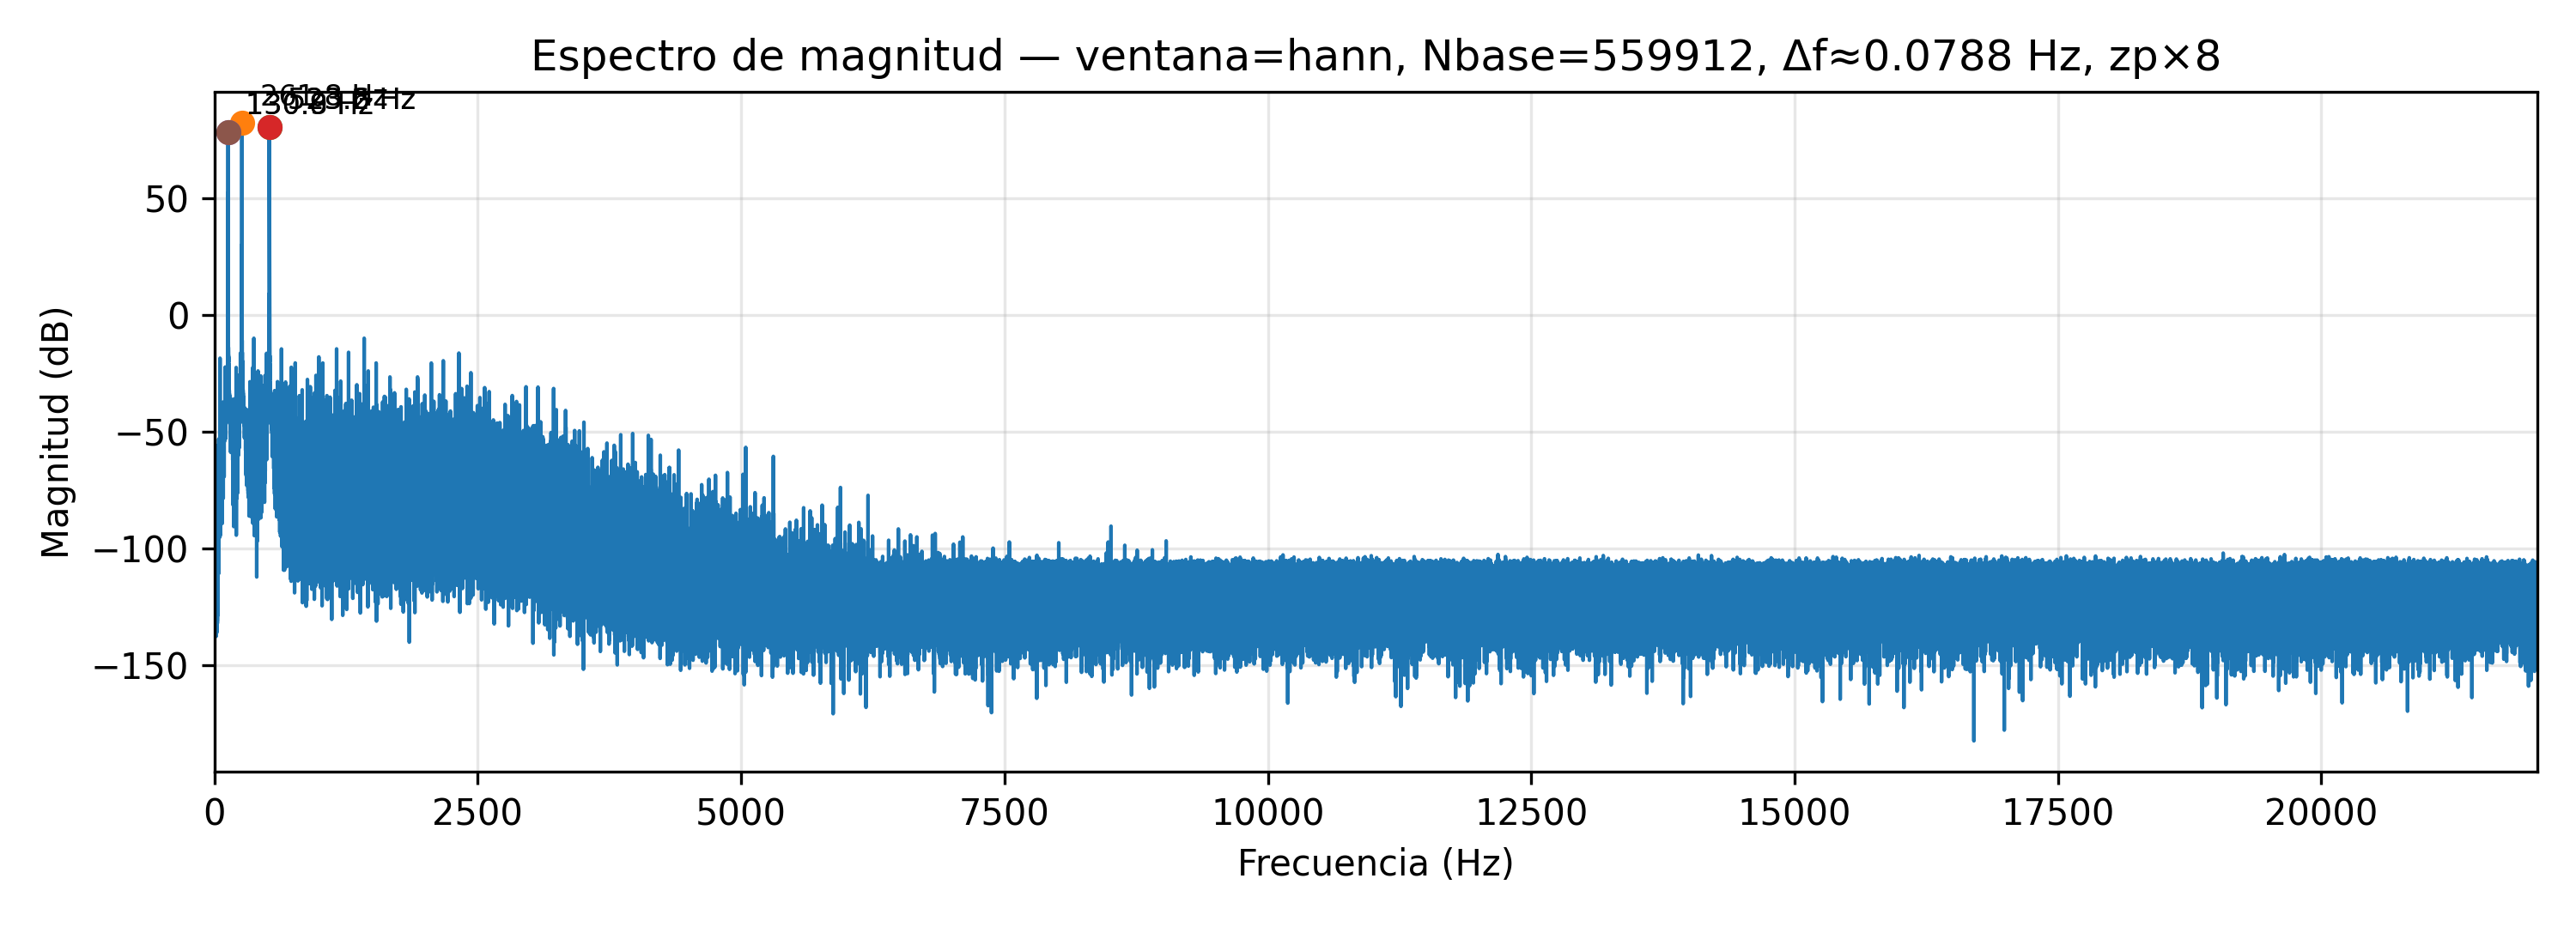
\includegraphics[width=0.95\linewidth]{../Codigo_Fuente/figs/magnitude_db_zoom.png}
  \caption{FFT por símbolo (vista de magnitud en dB, zoom alrededor de \(f_0\) y \(f_1\)). El pico dominante determina el bit recibido.}
  \label{fig:demod-freq}
\end{figure}

% (Opcional) espectrograma para visualizar saltos de frecuencia por símbolo
\begin{figure}[H]
  \centering
  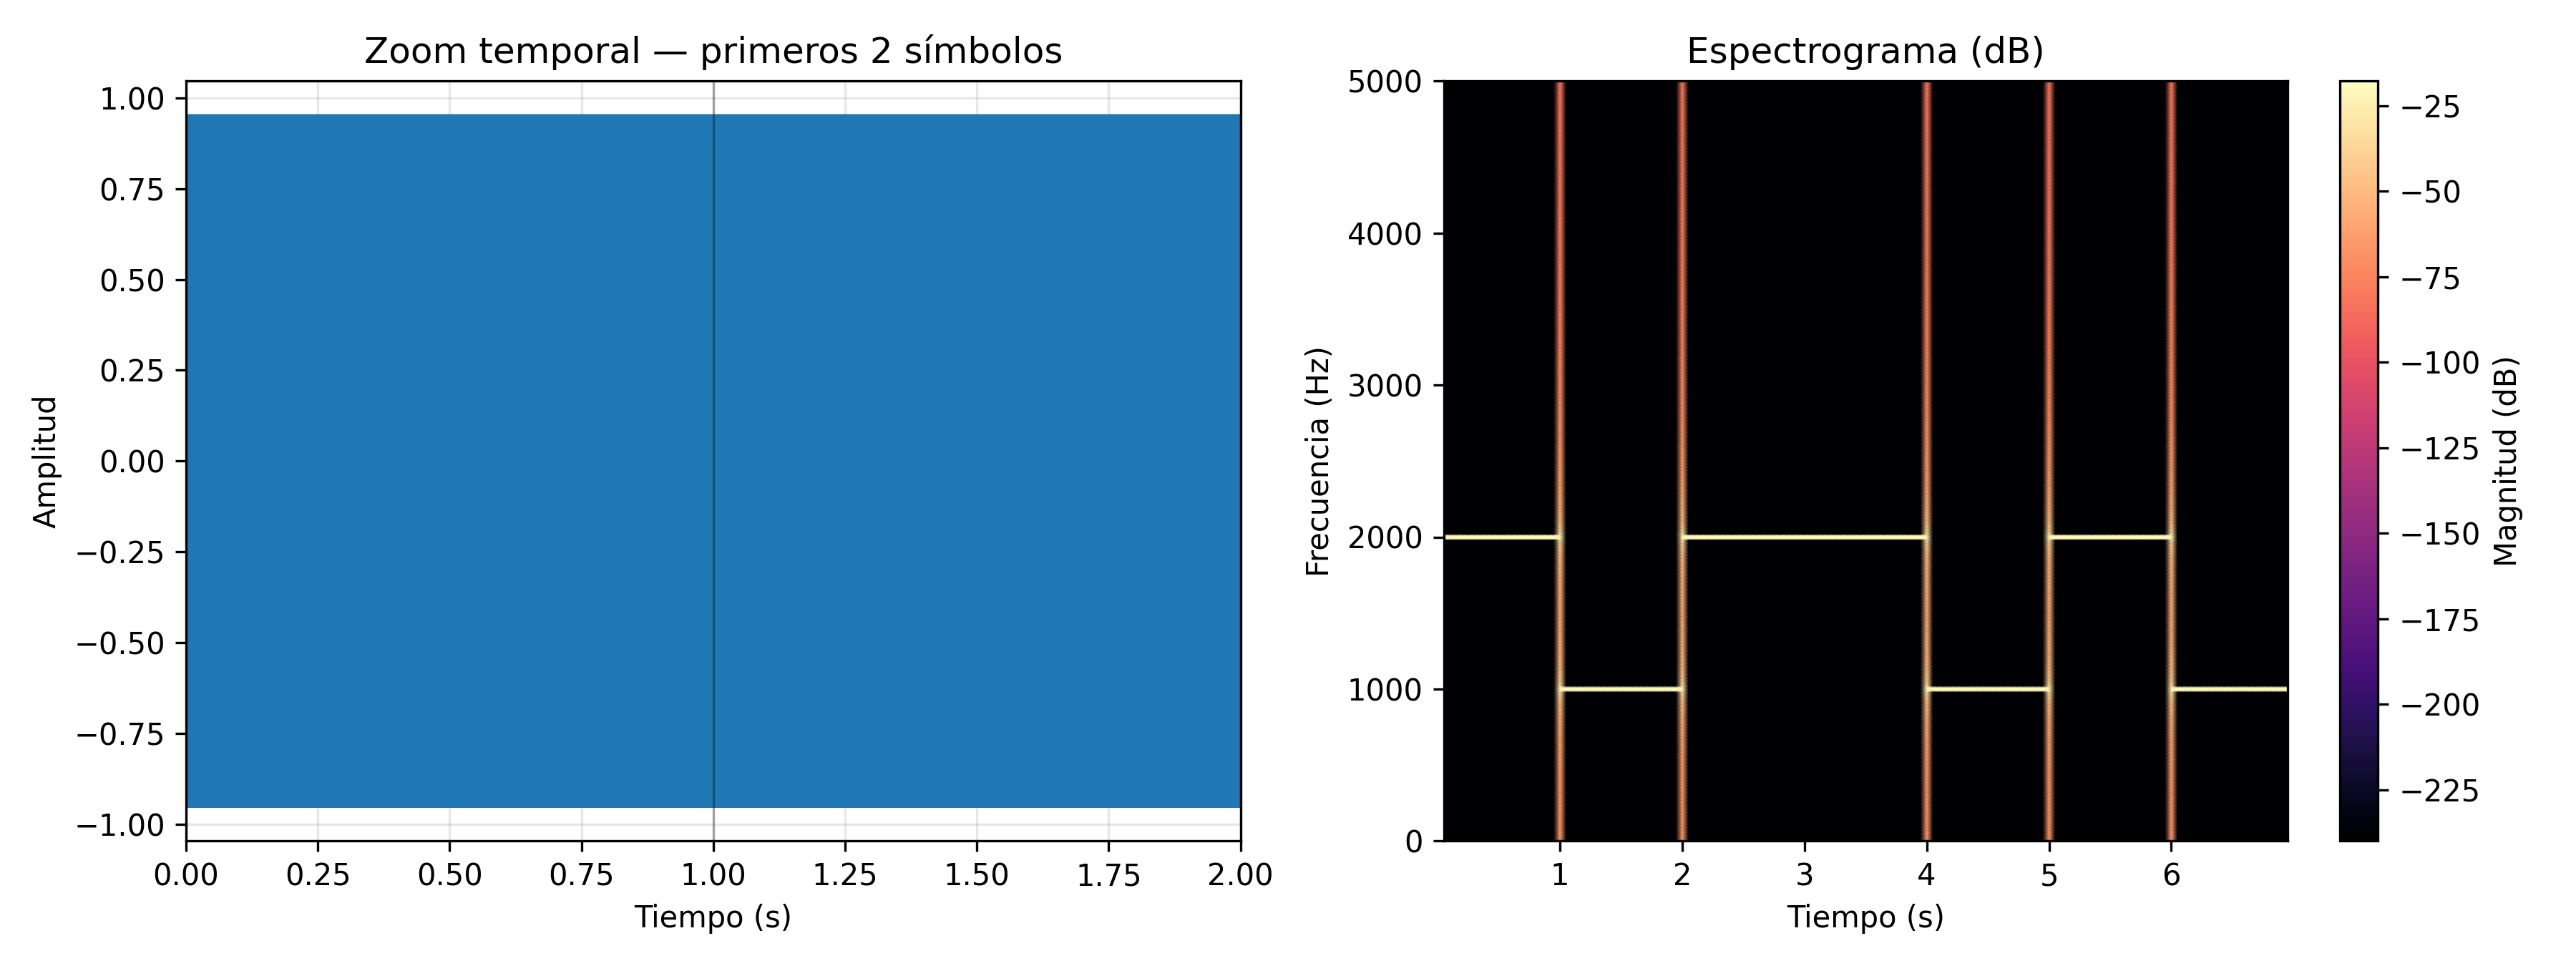
\includegraphics[width=0.95\linewidth]{../Codigo_Fuente/figs/fsk_demo_zoom_spectrogram.png}
  \caption{Espectrograma (ventana Hann). Se aprecian los saltos entre \(f_0\) y \(f_1\) por símbolo.}
  \label{fig:fsk-spec}
\end{figure}

\subsubsection{Discusión de desempeño}
En la corrida base sin ruido y con sincronización perfecta de símbolos, la separación \(|f_1-f_0|=1000\) Hz y la resolución \(\Delta f\approx 10\) Hz garantizan detección robusta. Se obtuvo BER=0 sobre 7 símbolos (patrón 1011010). La ventana de Hann reduce fuga espectral y el \emph{zero padding} (\(zp=2\)) densifica la malla para una lectura de picos más estable, sin cambiar la resolución física.
\begin{itemize}
  \item Recuperación de banda base: correcta (picos nítidos en \(f_0\)/\(f_1\); coincidencia bit a bit).
  \item Distorsión/ruido: despreciables en esta demo (canal ideal).
  \item Sincronía: el método asume fronteras de símbolo conocidas; desalineaciones degradan la decisión FFT.
  \item Limitaciones: no se modeló canal (ruido, desvanecimiento), \(\Delta f\) fijada por \(T_b\), y detector no coherente simple por distancia a \(f_0\)/\(f_1\).
\end{itemize}
% ...existing code...

    
% ====== Referencias ======
\newpage
\printbibliography

\end{document}